\documentclass[sigplan,10pt,review,anonymous]{acmart}\settopmatter{printfolios=true,printccs=false,printacmref=false}
\settopmatter{printacmref=false}
\setcopyright{none}
\renewcommand\footnotetextcopyrightpermission[1]{}
\pagestyle{plain}

%% Some recommended packages.
\usepackage{booktabs}   %% For formal tables:
                        %% http://ctan.org/pkg/booktabs
\usepackage{subcaption} %% For complex figures with subfigures/subcaptions
                        %% http://ctan.org/pkg/subcaption


%%%%%%%%%%%%%%%%%%%%%%%%%%%%%%%%%%%%%%%%%%%%%%%%%%%%%%%%%%%%%%%%%%%%%%%
%% Custom definitions
%%%%%%%%%%%%%%%%%%%%%%%%%%%%%%%%%%%%%%%%%%%%%%%%%%%%%%%%%%%%%%%%%%%%%%%

\usepackage{balance}
%\usepackage{url}
\usepackage{enumitem}
\usepackage{hyperref}
\usepackage{listings}
\usepackage{xspace}
\usepackage{cleveref}
\usepackage{multirow}
\usepackage{microtype}
\usepackage{soul,xcolor}
\usepackage{mathpartir}
\usepackage{amsmath,amsthm}
\usepackage[utf8]{inputenc}
\DeclareUnicodeCharacter{2200}{\ensuremath{\forall}} % ∀
\DeclareUnicodeCharacter{2083}{\ensuremath{_3}} % ₃
\DeclareUnicodeCharacter{2102}{\ensuremath{\mathbb{C}}} % ℂ
\DeclareUnicodeCharacter{D7}{\ensuremath{\times}} % ×
\DeclareUnicodeCharacter{2287}{\ensuremath{\supseteq}} % ⊇
\DeclareUnicodeCharacter{2208}{\ensuremath{\in}} % ∈
\DeclareUnicodeCharacter{230A}{\ensuremath{\lfloor{}}} % ⌊
\DeclareUnicodeCharacter{391}{\ensuremath{\Alpha}} % Α
\DeclareUnicodeCharacter{2293}{\ensuremath{\sqcap}} % ⊓
\DeclareUnicodeCharacter{1D502}{\ensuremath{\mathcal{y}}} % 𝔂
\DeclareUnicodeCharacter{395}{\ensuremath{\Epsilon}} % Ε
\DeclareUnicodeCharacter{2297}{\ensuremath{\otimes}} % ⊗
\DeclareUnicodeCharacter{399}{\ensuremath{\Iota}} % Ι
\DeclareUnicodeCharacter{2218}{\ensuremath{\circ}} % ∘
\DeclareUnicodeCharacter{229B}{\ensuremath{?}} % ⊛
\DeclareUnicodeCharacter{211A}{\ensuremath{\mathbb{Q}}} % ℚ
\DeclareUnicodeCharacter{39D}{\ensuremath{\Nu}} % Ν
\DeclareUnicodeCharacter{3A1}{\ensuremath{\Rho}} % Ρ
\DeclareUnicodeCharacter{3A5}{\ensuremath{\Upsilon}} % Υ
\DeclareUnicodeCharacter{22A7}{\ensuremath{\models}} % ⊧
\DeclareUnicodeCharacter{3A9}{\ensuremath{\Omega}} % Ω
\DeclareUnicodeCharacter{2228}{\ensuremath{\lor}} % ∨
\DeclareUnicodeCharacter{3B1}{\ensuremath{\alpha}} % α
\DeclareUnicodeCharacter{B3}{\ensuremath{^3}} % ³
\DeclareUnicodeCharacter{3B5}{\ensuremath{\epsilon}} % ε
\DeclareUnicodeCharacter{3B9}{\ensuremath{\iota}} % ι
\DeclareUnicodeCharacter{3BD}{\ensuremath{\nu}} % ν
\DeclareUnicodeCharacter{1D53E}{\ensuremath{\mathbb{G}}} % 𝔾
\DeclareUnicodeCharacter{3C1}{\ensuremath{\rho}} % ρ
\DeclareUnicodeCharacter{22C3}{\ensuremath{\bigcup}} % ⋃
\DeclareUnicodeCharacter{1D542}{\ensuremath{\mathbb{K}}} % 𝕂
\DeclareUnicodeCharacter{3C5}{\ensuremath{\upsilon}} % υ
\DeclareUnicodeCharacter{1D546}{\ensuremath{\mathbb{O}}} % 𝕆
\DeclareUnicodeCharacter{3C9}{\ensuremath{\omega}} % ω
\DeclareUnicodeCharacter{1D54A}{\ensuremath{\mathbb{S}}} % 𝕊
\DeclareUnicodeCharacter{1D54E}{\ensuremath{\mathbb{W}}} % 𝕎
\DeclareUnicodeCharacter{1D4D3}{\ensuremath{\mathcal{D}}} % 𝓓
\DeclareUnicodeCharacter{1D552}{\ensuremath{\mathbb{a}}} % 𝕒
\DeclareUnicodeCharacter{1D4D7}{\ensuremath{\mathcal{H}}} % 𝓗
\DeclareUnicodeCharacter{1D556}{\ensuremath{\mathbb{e}}} % 𝕖
\DeclareUnicodeCharacter{1D4DB}{\ensuremath{\mathcal{L}}} % 𝓛
\DeclareUnicodeCharacter{1D55A}{\ensuremath{\mathbb{i}}} % 𝕚
\DeclareUnicodeCharacter{1D4DF}{\ensuremath{\mathcal{P}}} % 𝓟
\DeclareUnicodeCharacter{1D55E}{\ensuremath{\mathbb{m}}} % 𝕞
\DeclareUnicodeCharacter{1D4E3}{\ensuremath{\mathcal{T}}} % 𝓣
\DeclareUnicodeCharacter{1D562}{\ensuremath{\mathbb{q}}} % 𝕢
\DeclareUnicodeCharacter{2264}{\ensuremath{\leq}} % ≤
\DeclareUnicodeCharacter{1D4E7}{\ensuremath{\mathcal{X}}} % 𝓧
\DeclareUnicodeCharacter{1D566}{\ensuremath{\mathbb{u}}} % 𝕦
\DeclareUnicodeCharacter{1D4EB}{\ensuremath{\mathcal{b}}} % 𝓫
\DeclareUnicodeCharacter{1D56A}{\ensuremath{\mathbb{y}}} % 𝕪
\DeclareUnicodeCharacter{1D4EF}{\ensuremath{\mathcal{f}}} % 𝓯
\DeclareUnicodeCharacter{2070}{\ensuremath{^0}} % ⁰
\DeclareUnicodeCharacter{1D4F3}{\ensuremath{\mathcal{j}}} % 𝓳
\DeclareUnicodeCharacter{2074}{\ensuremath{^4}} % ⁴
\DeclareUnicodeCharacter{1D4F7}{\ensuremath{\mathcal{n}}} % 𝓷
\DeclareUnicodeCharacter{27F9}{\ensuremath{\Longrightarrow}} % ⟹
\DeclareUnicodeCharacter{1D4FB}{\ensuremath{\mathcal{r}}} % 𝓻
\DeclareUnicodeCharacter{1D4FF}{\ensuremath{\mathcal{v}}} % 𝓿
\DeclareUnicodeCharacter{1D501}{\ensuremath{\mathcal{x}}} % 𝔁
\DeclareUnicodeCharacter{2080}{\ensuremath{_0}} % ₀
\DeclareUnicodeCharacter{2203}{\ensuremath{\exists}} % ∃
\DeclareUnicodeCharacter{2084}{\ensuremath{_4}} % ₄
\DeclareUnicodeCharacter{2309}{\ensuremath{\rceil{}}} % ⌉
\DeclareUnicodeCharacter{210D}{\ensuremath{\mathbb{H}}} % ℍ
\DeclareUnicodeCharacter{392}{\ensuremath{\Beta}} % Β
\DeclareUnicodeCharacter{2115}{\ensuremath{\mathbb{N}}} % ℕ
\DeclareUnicodeCharacter{2294}{\ensuremath{\sqcup}} % ⊔
\DeclareUnicodeCharacter{396}{\ensuremath{\Zeta}} % Ζ
\DeclareUnicodeCharacter{2119}{\ensuremath{\mathbb{P}}} % ℙ
\DeclareUnicodeCharacter{39A}{\ensuremath{\Kappa}} % Κ
\DeclareUnicodeCharacter{211D}{\ensuremath{\mathbb{R}}} % ℝ
\DeclareUnicodeCharacter{39E}{\ensuremath{\Xi}} % Ξ
\DeclareUnicodeCharacter{22A4}{\ensuremath{\top}} % ⊤
\DeclareUnicodeCharacter{2227}{\ensuremath{\land}} % ∧
\DeclareUnicodeCharacter{3A6}{\ensuremath{\Phi}} % Φ
\DeclareUnicodeCharacter{3B2}{\ensuremath{\beta}} % β
\DeclareUnicodeCharacter{3B6}{\ensuremath{\zeta}} % ζ
\DeclareUnicodeCharacter{1D539}{\ensuremath{\mathbb{B}}} % 𝔹
\DeclareUnicodeCharacter{3BA}{\ensuremath{\kappa}} % κ
\DeclareUnicodeCharacter{1D53D}{\ensuremath{\mathbb{F}}} % 𝔽
\DeclareUnicodeCharacter{3BE}{\ensuremath{\xi}} % ξ
\DeclareUnicodeCharacter{1D541}{\ensuremath{\mathbb{J}}} % 𝕁
\DeclareUnicodeCharacter{22C0}{\ensuremath{\bigland}} % ⋀
\DeclareUnicodeCharacter{2243}{\ensuremath{\simeq}} % ≃
\DeclareUnicodeCharacter{3C6}{\ensuremath{\phi}} % φ
\DeclareUnicodeCharacter{1D54D}{\ensuremath{\mathbb{V}}} % 𝕍
\DeclareUnicodeCharacter{1D4D0}{\ensuremath{\mathcal{A}}} % 𝓐
\DeclareUnicodeCharacter{21D2}{\ensuremath{\Rightarrow}} % ⇒
\DeclareUnicodeCharacter{1D555}{\ensuremath{\mathbb{d}}} % 𝕕
\DeclareUnicodeCharacter{1D4D4}{\ensuremath{\mathcal{E}}} % 𝓔
\DeclareUnicodeCharacter{1D559}{\ensuremath{\mathbb{h}}} % 𝕙
\DeclareUnicodeCharacter{1D4D8}{\ensuremath{\mathcal{I}}} % 𝓘
\DeclareUnicodeCharacter{1D55D}{\ensuremath{\mathbb{l}}} % 𝕝
\DeclareUnicodeCharacter{1D4DC}{\ensuremath{\mathcal{M}}} % 𝓜
\DeclareUnicodeCharacter{1D561}{\ensuremath{\mathbb{p}}} % 𝕡
\DeclareUnicodeCharacter{1D4E0}{\ensuremath{\mathcal{Q}}} % 𝓠
\DeclareUnicodeCharacter{1D565}{\ensuremath{\mathbb{t}}} % 𝕥
\DeclareUnicodeCharacter{1D4E4}{\ensuremath{\mathcal{U}}} % 𝓤
\DeclareUnicodeCharacter{27E6}{\ensuremath{\llbracket}} % ⟦
\DeclareUnicodeCharacter{1D569}{\ensuremath{\mathbb{x}}} % 𝕩
\DeclareUnicodeCharacter{1D4E8}{\ensuremath{\mathcal{Y}}} % 𝓨
\DeclareUnicodeCharacter{1D4EC}{\ensuremath{\mathcal{c}}} % 𝓬
\DeclareUnicodeCharacter{1D4F0}{\ensuremath{\mathcal{g}}} % 𝓰
\DeclareUnicodeCharacter{1D4F4}{\ensuremath{\mathcal{k}}} % 𝓴
\DeclareUnicodeCharacter{27F6}{\ensuremath{\longrightarrow}} % ⟶
\DeclareUnicodeCharacter{1D4F8}{\ensuremath{\mathcal{o}}} % 𝓸
\DeclareUnicodeCharacter{207B}{\ensuremath{^{-}}} % ⁻
\DeclareUnicodeCharacter{1D4FC}{\ensuremath{\mathcal{s}}} % 𝓼
\DeclareUnicodeCharacter{2081}{\ensuremath{_1}} % ₁
\DeclareUnicodeCharacter{1D500}{\ensuremath{\mathcal{w}}} % 𝔀
\DeclareUnicodeCharacter{2202}{\ensuremath{\partial}} % ∂
\DeclareUnicodeCharacter{2A06}{\ensuremath{\bigsqcup}} % ⨆
\DeclareUnicodeCharacter{2308}{\ensuremath{\lceil{}}} % ⌈
\DeclareUnicodeCharacter{2291}{\ensuremath{\sqsubseteq}} % ⊑
\DeclareUnicodeCharacter{393}{\ensuremath{\Gamma}} % Γ
\DeclareUnicodeCharacter{2295}{\ensuremath{\oplus}} % ⊕
\DeclareUnicodeCharacter{397}{\ensuremath{\Eta}} % Η
\DeclareUnicodeCharacter{39B}{\ensuremath{\Lambda}} % Λ
\DeclareUnicodeCharacter{39F}{\ensuremath{\Omicron}} % Ο
\DeclareUnicodeCharacter{3A3}{\ensuremath{\Sigma}} % Σ
\DeclareUnicodeCharacter{22A5}{\ensuremath{\bot}} % ⊥
\DeclareUnicodeCharacter{2124}{\ensuremath{\mathbb{Z}}} % ℤ
\DeclareUnicodeCharacter{3A7}{\ensuremath{\Chi}} % Χ
\DeclareUnicodeCharacter{2026}{\ensuremath{\dots}} % …
\DeclareUnicodeCharacter{1F4A9}{\ensuremath{\LaTeX}} % 💩
\DeclareUnicodeCharacter{222A}{\ensuremath{\cup}} % ∪
\DeclareUnicodeCharacter{3B3}{\ensuremath{\gamma}} % γ
\DeclareUnicodeCharacter{3B7}{\ensuremath{\eta}} % η
\DeclareUnicodeCharacter{B9}{\ensuremath{^1}} % ¹
\DeclareUnicodeCharacter{1D538}{\ensuremath{\mathbb{A}}} % 𝔸
\DeclareUnicodeCharacter{3BB}{\ensuremath{\lambda}} % λ
\DeclareUnicodeCharacter{1D53C}{\ensuremath{\mathbb{E}}} % 𝔼
\DeclareUnicodeCharacter{3BF}{\ensuremath{\omicron}} % ο
\DeclareUnicodeCharacter{22C1}{\ensuremath{\biglor}} % ⋁
\DeclareUnicodeCharacter{1D540}{\ensuremath{\mathbb{I}}} % 𝕀
\DeclareUnicodeCharacter{3C3}{\ensuremath{\sigma}} % σ
\DeclareUnicodeCharacter{22C5}{\ensuremath{\cdot}} % ⋅
\DeclareUnicodeCharacter{1D544}{\ensuremath{\mathbb{M}}} % 𝕄
\DeclareUnicodeCharacter{3C7}{\ensuremath{\chi}} % χ
\DeclareUnicodeCharacter{1D54C}{\ensuremath{\mathbb{U}}} % 𝕌
\DeclareUnicodeCharacter{1D4D1}{\ensuremath{\mathcal{B}}} % 𝓑
\DeclareUnicodeCharacter{1D550}{\ensuremath{\mathbb{Y}}} % 𝕐
\DeclareUnicodeCharacter{1D4D5}{\ensuremath{\mathcal{F}}} % 𝓕
\DeclareUnicodeCharacter{1D554}{\ensuremath{\mathbb{c}}} % 𝕔
\DeclareUnicodeCharacter{1D4D9}{\ensuremath{\mathcal{J}}} % 𝓙
\DeclareUnicodeCharacter{1D558}{\ensuremath{\mathbb{g}}} % 𝕘
\DeclareUnicodeCharacter{1D4DD}{\ensuremath{\mathcal{N}}} % 𝓝
\DeclareUnicodeCharacter{1D55C}{\ensuremath{\mathbb{k}}} % 𝕜
\DeclareUnicodeCharacter{1D4E1}{\ensuremath{\mathcal{R}}} % 𝓡
\DeclareUnicodeCharacter{1D560}{\ensuremath{\mathbb{o}}} % 𝕠
\DeclareUnicodeCharacter{1D4E5}{\ensuremath{\mathcal{V}}} % 𝓥
\DeclareUnicodeCharacter{1D564}{\ensuremath{\mathbb{s}}} % 𝕤
\DeclareUnicodeCharacter{27E7}{\ensuremath{\rrbracket}} % ⟧
\DeclareUnicodeCharacter{1D4E9}{\ensuremath{\mathcal{Z}}} % 𝓩
\DeclareUnicodeCharacter{1D568}{\ensuremath{\mathbb{w}}} % 𝕨
\DeclareUnicodeCharacter{1D4ED}{\ensuremath{\mathcal{d}}} % 𝓭
\DeclareUnicodeCharacter{1D4F1}{\ensuremath{\mathcal{h}}} % 𝓱
\DeclareUnicodeCharacter{2192}{\ensuremath{\rightarrow}} % →
\DeclareUnicodeCharacter{1D4F5}{\ensuremath{\mathcal{l}}} % 𝓵
\DeclareUnicodeCharacter{1D4F9}{\ensuremath{\mathcal{p}}} % 𝓹
\DeclareUnicodeCharacter{207A}{\ensuremath{^{+}}} % ⁺
\DeclareUnicodeCharacter{1D4FD}{\ensuremath{\mathcal{t}}} % 𝓽
\DeclareUnicodeCharacter{1D503}{\ensuremath{\mathcal{z}}} % 𝔃
\DeclareUnicodeCharacter{2082}{\ensuremath{_2}} % ₂
\DeclareUnicodeCharacter{2A05}{\ensuremath{\bigsqcap}} % ⨅
\DeclareUnicodeCharacter{2286}{\ensuremath{\subseteq}} % ⊆
\DeclareUnicodeCharacter{230B}{\ensuremath{\rfloor{}}} % ⌋
\DeclareUnicodeCharacter{2292}{\ensuremath{\sqsupseteq}} % ⊒
\DeclareUnicodeCharacter{394}{\ensuremath{\Delta}} % Δ
\DeclareUnicodeCharacter{398}{\ensuremath{\Theta}} % Θ
\DeclareUnicodeCharacter{39C}{\ensuremath{\Mu}} % Μ
\DeclareUnicodeCharacter{3A0}{\ensuremath{\Pi}} % Π
\DeclareUnicodeCharacter{22A2}{\ensuremath{\vdash}} % ⊢
\DeclareUnicodeCharacter{3A4}{\ensuremath{\Tau}} % Τ
\DeclareUnicodeCharacter{2229}{\ensuremath{\cap}} % ∩
\DeclareUnicodeCharacter{3A8}{\ensuremath{\Psi}} % Ψ
\DeclareUnicodeCharacter{B2}{\ensuremath{^2}} % ²
\DeclareUnicodeCharacter{3B4}{\ensuremath{\delta}} % δ
\DeclareUnicodeCharacter{3B8}{\ensuremath{\theta}} % θ
\DeclareUnicodeCharacter{1D53B}{\ensuremath{\mathbb{D}}} % 𝔻
\DeclareUnicodeCharacter{3BC}{\ensuremath{\mu}} % μ
\DeclareUnicodeCharacter{3C0}{\ensuremath{\pi}} % π
\DeclareUnicodeCharacter{1D543}{\ensuremath{\mathbb{L}}} % 𝕃
\DeclareUnicodeCharacter{22C2}{\ensuremath{\bigcap}} % ⋂
\DeclareUnicodeCharacter{2245}{\ensuremath{\cong}} % ≅
\DeclareUnicodeCharacter{3C4}{\ensuremath{\tau}} % τ
\DeclareUnicodeCharacter{3C8}{\ensuremath{\psi}} % ψ
\DeclareUnicodeCharacter{1D54B}{\ensuremath{\mathbb{T}}} % 𝕋
\DeclareUnicodeCharacter{1D54F}{\ensuremath{\mathbb{X}}} % 𝕏
\DeclareUnicodeCharacter{1D553}{\ensuremath{\mathbb{b}}} % 𝕓
\DeclareUnicodeCharacter{1D4D2}{\ensuremath{\mathcal{C}}} % 𝓒
\DeclareUnicodeCharacter{1D557}{\ensuremath{\mathbb{f}}} % 𝕗
\DeclareUnicodeCharacter{1D4D6}{\ensuremath{\mathcal{G}}} % 𝓖
\DeclareUnicodeCharacter{1D55B}{\ensuremath{\mathbb{j}}} % 𝕛
\DeclareUnicodeCharacter{1D4DA}{\ensuremath{\mathcal{K}}} % 𝓚
\DeclareUnicodeCharacter{1D55F}{\ensuremath{\mathbb{n}}} % 𝕟
\DeclareUnicodeCharacter{1D4DE}{\ensuremath{\mathcal{O}}} % 𝓞
\DeclareUnicodeCharacter{2261}{\ensuremath{\equiv}} % ≡
\DeclareUnicodeCharacter{1D563}{\ensuremath{\mathbb{r}}} % 𝕣
\DeclareUnicodeCharacter{1D4E2}{\ensuremath{\mathcal{S}}} % 𝓢
\DeclareUnicodeCharacter{2265}{\ensuremath{\geq}} % ≥
\DeclareUnicodeCharacter{1D567}{\ensuremath{\mathbb{v}}} % 𝕧
\DeclareUnicodeCharacter{1D4E6}{\ensuremath{\mathcal{W}}} % 𝓦
\DeclareUnicodeCharacter{1D56B}{\ensuremath{\mathbb{z}}} % 𝕫
\DeclareUnicodeCharacter{1D4EA}{\ensuremath{\mathcal{a}}} % 𝓪
\DeclareUnicodeCharacter{1D4EE}{\ensuremath{\mathcal{e}}} % 𝓮
\DeclareUnicodeCharacter{1D4F2}{\ensuremath{\mathcal{i}}} % 𝓲
\DeclareUnicodeCharacter{1D4F6}{\ensuremath{\mathcal{m}}} % 𝓶
\DeclareUnicodeCharacter{1D4FA}{\ensuremath{\mathcal{q}}} % 𝓺
\DeclareUnicodeCharacter{1D4FE}{\ensuremath{\mathcal{u}}} % 𝓾

\usepackage{mathtools}
\usepackage{tikz}
\usetikzlibrary{calc,decorations.pathmorphing,shapes}
\usepackage{stmaryrd}
\usepackage{adjustbox}

\newcommand{\rot}[2][70]{\adjustbox{angle=#1}{\textbf{#2}}}

\crefformat{section}{§#2#1#3}
\newtheorem{theorem}{Theorem}
\newtheorem{definition}[theorem]{Definition}

\newenvironment{nop}{}{}
\newenvironment{smathpar}{
\begin{nop}\small\begin{mathpar}}{
\end{mathpar}\end{nop}\ignorespacesafterend}

\newcommand{\kc}[1]{{\color{red} {\it [KC says: #1]}}}
\newcommand{\am}[1]{{\color{blue} {\it [AM says: #1]}}}
\newcommand{\tk}[1]{{\color{blue} {\it [TK says: #1]}}}

\definecolor{Bittersweet}{rgb}{1.0, 0.44, 0.37}
\definecolor{MidnightBlue}{rgb}{0.0, 0.2, 0.4}
\definecolor{BrightBlue}{rgb}{0.0, 0.2, 0.7}
\definecolor{byzantine}{rgb}{0.74, 0.2, 0.64}
\definecolor{caribbeangreen}{rgb}{0.0, 0.8, 0.6}

\lstset{
      language=caml,
      basicstyle=\ttfamily\footnotesize,
      flexiblecolumns=false,
      tabsize=2,
      escapechar={<@}{@>},
      basewidth={0.5em,0.45em},
      aboveskip={3pt},
      belowskip={3pt},
      breaklines = true,
      breakatwhitespace = true,
      keywordstyle=\color{Bittersweet}\bfseries,
      commentstyle=\color{blue}\itshape,
      stringstyle=\color{MidnightBlue},
      keywords=[2]{},
      keywordstyle=[2]\color{byzantine}\bfseries,
      keywords=[3]{eff,effect,perform,continue,discontinue,continuation,
                   clone_continuation},
      keywordstyle=[3]\color{caribbeangreen}\bfseries,
      keywords=[4]{call,return,external},
      keywordstyle=[4]\color{Bittersweet}\bfseries,
      classoffset=1,
      upquote=true,
      keywordstyle=\color{byzantine}\bfseries,
      classoffset=0,
      mathescape=true,
      numberstyle=\tiny\color{gray},
      numbersep=5pt
}

\lstnewenvironment{code}[1][]
    { % \centering
      \lstset{
        basicstyle=\ttfamily\footnotesize,
        #1}%
      \csname lst@setfirstlabel\endcsname}
    { %\centering
      \csname lst@savefirstlabel\endcsname}

\lstMakeShortInline[columns=fullflexible,keepspaces]|

\setlength{\tabcolsep}{3pt}

%%%%%%%%%%%%%%%%%%%%%%%%%%%%%%%%%%%%%%%%%%%%%%%%%%%%%%%%%%%%%%%%%%%%%%%
%% Semantics definitions
%%%%%%%%%%%%%%%%%%%%%%%%%%%%%%%%%%%%%%%%%%%%%%%%%%%%%%%%%%%%%%%%%%%%%%%


\newcommand{\olam}[2]{\lambda^o #1. #2}
\newcommand{\llambda}{\lambda\!\!\lambda}
\newcommand{\clam}[2]{\lambda^c #1. #2}
\newcommand{\lam}[2]{\Lambda #1. #2}

\newcommand{\env}{\epsilon}
\newcommand{\envext}[3]{#1[#2 \mapsto #3]}

\newcommand{\oclos}[3]{\llparenthesis \olam{#1}{#2}, #3 \rrparenthesis}
\newcommand{\cclos}[3]{\llparenthesis \clam{#1}{#2}, #3 \rrparenthesis}
\newcommand{\clos}[3]{\llparenthesis \lam{#1}{#2}, #3 \rrparenthesis}
\newcommand{\kw}[1]{\text{\bf #1}}
\newcommand{\effval}[2]{\textsf{eff} ~#1 ~#2}
\newcommand{\exnval}[1]{\textsf{exn} ~#1}

\newcommand{\handle}[2]{\kw{match} ~#1 ~\kw{with} ~#2}
\newcommand{\throw}[2]{\kw{raise} ~#1 ~#2}
\newcommand{\perform}[2]{\kw{perform} ~#1 ~#2}

\newcommand{\caseval}[2]{\kw{return}~#1 \mapsto #2}
\newcommand{\caseexn}[3]{\kw{exception} ~#1 ~#2 \mapsto #3}
\newcommand{\caseeff}[4]{\kw{effect} ~#1 ~#2 ~#3 \mapsto #4}

\newcommand{\farg}[2]{\langle #1 ~#2 \rangle_a}
\newcommand{\ffun}[1]{\langle #1 \rangle_f}
\newcommand{\faritha}[3]{\langle #1 ~#2 ~#3 \rangle_{b1}}
\newcommand{\farithb}[2]{\langle #1 ~#2 \rangle_{b2}}

\newcommand{\kcons}{\lhd}
\newcommand{\fiber}{\varphi}
\newcommand{\fl}{\psi} % Frame List
\newcommand{\hc}{\eta} % Handler Closure

\newcommand{\cstack}{\gamma} % C Stack
\newcommand{\ostack}{\omega} % OCaml Stack
\newcommand{\cstacka}[2]{\big \lceil #1, #2 \big \rceil_c} % C stack with arguments
\newcommand{\ostacka}[2]{\big \lceil #1, #2 \big \rceil_o} % OCaml stack with arguments
\newcommand{\ostackemp}{\bullet}
\newcommand{\stack}{\sigma}

\newcommand{\term}{\tau}
\newcommand{\config}{\mathfrak{C}}
\newcommand{\configa}[3]{\|#1,#2,#3\|}

\newcommand{\ostep}{\xrightarrow{o}}
\newcommand{\cstep}{\xrightarrow{c}}
\newcommand{\step}{\rightarrow}

\begin{document}

\title{Retrofitting Effect Handlers onto OCaml}

\begin{abstract}
Effect handlers have been gathering momentum as a mechanism
for modular programming with user-defined effects. The runtime semantics of
effect handlers allow for control flow
mechanisms such as first-class continuations, generators, async/await and coroutines to be composably expressed. We present a design and evaluate a
full-fledged efficient implementation of effect handlers for OCaml, an industrial-strength multi-paradigm programming language. Our implementation strives to maintain the existing performance profile of conventional OCaml code, particularly in the domain of systems and toolchain programming. Retrofitting effect handlers onto OCaml is challenging since OCaml does currently not have any non-local control flow mechanisms other than exceptions. Our implementation of
effect handlers for OCaml: {\em (i)} imposes negligible overhead on code that does not use
effect handlers; {\em (ii)} remains compatible with program analysis tools that inspect the
stack; and {\em (iii)} is efficient for new code that makes use of effect handlers.
\end{abstract}

\maketitle

\section{Introduction}

Effect handlers~\cite{Plotkin09} provide a modular foundation for user-defined
effects. The key idea is to separate the definition of the effectful operations
from their interpretations, which are defined by \emph{handlers} of the
effects. For example,
%
\begin{lstlisting}
effect Read : in_channel -> string
\end{lstlisting}
%
declares an \emph{effect} |Read|, which is parameterised with an input channel
of type |in_channel|, which when \emph{performed} returns a |string| value. A
computation can perform the |Read| effect without knowing how the |Read| effect
is implemented. This computation may be enclosed by different handlers that
interpret |Read| differently. For example, |Read| may be implemented by
performing a blocking read on the input channel or performing the read
asynchronously by offloading it to an event loop such as |libuv|. Thanks to the
separation of effectful operations from their interpretations, effect handlers
enable new approaches to modular programming.

\subsection{An effectful calculator}

Effect handlers provide a structured
form of delimited continuations~\cite{Danvy90} that enables
non-local control-flow mechanisms such as resumable exceptions, coroutines,
generators and asynchronous I/O to be composably expressed. For example,
consider the task of handling division-by-zero in a calculator
application. Different calculators handle division-by-zero differently. In the
iOS 13 Calculator (|iOS|), |0/0| returns |Error|. In the Google
search calculator (|gsearch|) |0/0| returns |Error|, but for
|n!=0| the |n/0| returns |Infinity| with the same sign as |n|.
How do we capture all these different behaviours without changing the evaluator?

Common Lisp Conditions~\cite{Steele90} are an elegant way to solve this
problem. Unlike exceptions where the library decides whether an error is fatal
or not, conditions allow the client of the library to make that decision.
Conditions provide a \emph{restart} mechanism for non-fatal errors to resume
execution from the point where the condition was signalled. On
division-by-zero, the calculator signals the handler and lets the handler
decide the course of action based on the desired semantics. We now implement
this using effect handlers in OCaml syntax:

\begin{lstlisting}[numbers=left]
type sign = P | N
type val = Z of int | Error | Inf of sign
type exp = Val of val | ... | Div of exp*exp
effect DivBy0 : int -> val
let rec eval e =
  match e with
  | Val v -> v
  | ...
  | Div (e1,e2) ->
    match eval e1, eval e2 with
    | Z v1, Z v2 ->
        if v2 = 0 then perform (DivBy0 v1)
        else Z (v1/v2)
    | Error, _ -> Error | Inf s, _ -> Inf s
    | ...
let (/) n d = Div (Val (Z n), Val (Z d))
\end{lstlisting}

Line 4 declares an effect |DivBy0| that is parameterised by an integer,
which when performed returns the result of division-by-zero. If the denominator
is 0, then we perform the |DivBy0| effect with the numerator value (line 12) so that
the context may decide the return value. We obtain the |iOS| semantics by
wrapping the evaluator with this handler:
\begin{lstlisting}
let ios e = match eval e with
| v -> v
| effect (DivBy0 _) k -> continue k Error
\end{lstlisting}
If the evaluator returns a value, we simply return that. If the evaluator
performs the |DivBy0| effect, we catch the effect in the pattern match along with
the continuation |k| of the corresponding |perform| \emph{delimited} by this
handler. For |iOS|, we |continue| the suspended computation with an
|Error| value and the computation |ios(1/0)| returns |Error|.
We can get the |gsearch| semantics by enclosing the evaluator in this handler:
\begin{lstlisting}
let gsearch e = match eval e with
| v -> v
| effect (DivBy0 v) k ->
		if v = 0 then continue k Error
		else if v > 0 then continue k (Inf P)
		else continue k (Inf N)
\end{lstlisting}
Executing |gsearch(1/0)| returns positive infinity (|Inf P|).

\subsection{Asynchronous I/O}
\label{sec:aio}

We can modularly extend the calculator to read user input using the |Read|
effect defined earlier as follows:
\begin{lstlisting}
type exp = ... | Inp
effect Read : in_channel -> string
let rec eval e = match e with
| ...
| Inp -> int_of_string (perform (Read stdin))
\end{lstlisting}
The |Read| effect can then be handled by another handler enclosing the
division-by-zero handler:
\begin{lstlisting}
let run e = match gsearch e with
| v -> v
| effect (Read chan) k ->
		register_async_input_line (chan, k);
		continue (get_ui_k ()) ()
\end{lstlisting}
\noindent which registers the read operation to be performed asynchronously
with the continuation as the callback. Subsequently, it resumes the
user-interface continuation so that the application remains responsive. Observe
that neither of the handlers needs to be aware of the other.

\subsection{Retrofitting effect handlers}

There are many research languages and libraries built around effect
handlers~\cite{Leijen14,Hillerstrom20,Pyro,Frank,Eff}. Unlike these efforts, our
goal is to retrofit effect handlers onto the OCaml programming language, which
has been in continuous use for the past 25 years in large codebases including
verification tools~\cite{everest,Coq}, mission critical software
systems~\cite{astree} and latency sensitive networked
applications~\cite{Madhavapeddy13}. OCaml is particularly favoured for its
competitive yet predictable performance, with a fast foreign-function interface
(FFI). It has excellent compatibility with program analysis tools such as debuggers
and profilers that utilise DWARF stack unwind tables~\cite{DWARF} to obtain a
backtrace. Our primary motivation for adding effect handlers to OCaml is to
support: {\em (i)} highly concurrent applications such as web servers using a
natural \emph{direct-style} as opposed to using callbacks; and {\em (ii)} efficient
nested parallel programs in the vein of Cilk~\cite{Cilk}, OpenMP~\cite{OpenMP},
X10~\cite{Charles05}, Intel TBB~\cite{IntelTBB}, and variants of Parallel
ML~\cite{MaPLe, Fluet10, Sivaramakrishnan14}.

OCaml currently does not support any non-local control flow mechanisms other
than exceptions. This makes it particularly challenging to implement the
delimited continuations necessary for effect handlers without sacrificing the
desirable properties of OCaml. One standard way of implementing continuations is
to use continuation-passing style (CPS) in the compiler's intermediate
representation (IR)~\cite{Leijen14}. If the compiler were to use CPS, then
reifying continuations in the source language is relatively straight-forward.
But OCaml does not use a CPS IR, and changing the OCaml compiler to utilise a CPS IR
would be an enormous undertaking that would affect the
performance profile of existing OCaml applications due to increased memory allocations as
continuation closures get allocated on the heap~\cite{Farvardin20}. Moreover,
with CPS, stack unwinding is meaningless and hence, we would lose compatibility
with tools that inspect the program stack. Hence, we choose not to use CPS
translation and represent continuations as call stacks.

The search for an expressive effect system that guarantees that all the effects
performed in the program are handled (\emph{effect safety}) in the presence of
advanced features such as polymorphism, modularity and generativity is an
active area of research~\cite{Leijen14, Biernacki19, Biernacki20,
Hillerstrom20}. We do not focus on this question in this paper, and our
implementation of effect handlers in OCaml does not guarantee effect safety.
For example, running |perform (Read stdin)| without an enclosing handler raises
|Unhandled| exception at the point of |perform|. We leave the question of
effect safety for future work.

\subsection{Requirements}
\label{sec:req}

We motivate our effect handler design based on the following ideal
requirements:

\if{0}
\begin{enumerate}[label=R\arabic*]
  \item \textbf{Backwards compatibility} A well-behaved OCaml program does not
    break under an OCaml extended with effect handlers. OCaml code that does not
    use effect handlers will pay negligible performance cost.
  \item \textbf{Tool compatibility} OCaml with effect handlers produce
    well-formed backtraces, and remains compatible with program analysis tools
    such as debuggers and profilers that inspect the stack using DWARF stack
    unwind tables.
  \item \textbf{Effect handler efficiency} In order to support
    highly-concurrent applications, the program must accommodate millions of
    continuations at the same time. Installing effect handlers, capturing and
    resuming continuations must be fast.
  \item \textbf{Forwards compatibility} While this work does not present an
    effect system, the design must be compatible with a future effect system
    for OCaml. As a cornerstone of modularity, we also want blocking I/O code
    to \emph{transparently} be made asynchronous with the help of effect
    handlers.
\end{enumerate}
\fi

\noindent \textbf{R1: Backwards compatibility.} A well-behaved OCaml program does
not break under an OCaml that is extended with effect handlers. OCaml code that does not
use effect handlers will pay negligible performance and memory cost.

\noindent \textbf{R2: Tool compatibility.} OCaml programs with effect handlers produce
well-formed backtraces and remain compatible with program analysis tools such
as debuggers and profilers that inspect the stack using DWARF unwind
tables.

\noindent \textbf{R3: Effect handler efficiency.} The program must accommodate millions of
continuations at the same time to support
highly-concurrent applications. Installing effect handlers, capturing and
resuming continuations must be fast.

\noindent \textbf{R4: Forwards compatibility.} While this work does not present an
effect system, the design must be compatible with a future effect system for
OCaml. As a cornerstone of modularity, we also want blocking I/O code to
\emph{transparently} be made asynchronous with the help of effect handlers.

The need to host millions of continuations at the same time rules out the use
of a large contiguous stack space as in C for continuations. Instead, we resort
to using small initial stacks and growing the stacks on demand. As a result,
OCaml functions, irrespective of whether they use effect handlers, need to
perform stack overflow checks and external C functions, which do not have stack
overflow checks, must be performed on a separate system stack. Additionally, we
must generate DWARF stack unwind tables for stacks that may be non-contiguous.
In this work, we develop the compiler and runtime support for implementing
efficient effect handlers for OCaml that satisfy these requirements.

Our work is also timely. The WebAssembly~\cite{Hass17} community group is
actively considering effect handlers as one of the mechanism for supporting
concurrency, asynchronous I/O and generators~\cite{WasmProposal}. Project
Loom~\cite{loom} is an OpenJDK project which adds virtual threads and delimited
continuations to Java. Swift concurrency roadmap~\cite{swift} includes
direct-style asynchronous programming and structured concurrency as milestones.
We believe that our design choices will inform similar choices to be made in the
other industrial-strength languages.

\subsection{Contributions}

Our contributions are to present:

\begin{itemize}
  \item the design and implementation of one-shot effect handlers for OCaml.
    Our design retains OCaml's compatibility with program analysis tools that
    inspect the stack using DWARF unwind tables. We have validated our DWARF
    unwind tables with the assistance of an automated validator
    tool~\cite{Bastian19}.
  \item a formal operational semantics for the effect handler implementation in
    OCaml.
	\item extensive evaluation which shows that our implementation has negligible
		impact on code that does not use effect handlers, and serves as an
		efficient foundation for scalable concurrent programming.
\end{itemize}

We have implemented effect handlers in a multicore extension of the OCaml
programming language. We call our implementation \textbf{Multicore OCaml} to
distinguish it from stock OCaml.

The rest of the paper is organized as follows. The next section describes the
details of stock OCaml program stack. In \S\ref{sec:refine}, we refine the
design further focussing on retrofitting effect handlers into a mainstream
\emph{systems} language. \S\ref{sec:semantics} presents the compilation scheme
and operational semantics semantics for Multicore OCaml effect handlers.
\S\ref{sec:impl} discusses the compiler and the runtime system support for
implementing effect handlers. \S\ref{sec:eval} presents extensive performance
evaluation of effect handlers against the goals set in \S\ref{sec:req}.
\S\ref{sec:related} and \S\ref{sec:conc} present the related work and the
conclusions.

\section{Background: OCaml Stacks}
\label{sec:stack}

\begin{figure*}
\begin{minipage}{0.30\linewidth}
  \begin{minipage}{\linewidth}
    \begin{lstlisting}[numbers=left]
external ocaml_to_c
  : unit -> int = "ocaml_to_c"
exception E1
exception E2
let c_to_ocaml () = raise E1
let _ = Callback.register
    "c_to_ocaml" c_to_ocaml
let omain () =
  try (* h1 *)
    try (* h2 *) ocaml_to_c ()
    | with E2 -> 0
  | with E1 -> 42;;
let _ = assert (omain () = 42)
    \end{lstlisting}
    \vspace{-2mm}
    \subcaption{\texttt{meander.ml}}
    \label{code:meander_ml}
  \end{minipage}
  \begin{minipage}{\linewidth}
    \begin{lstlisting}[language=c,numbers=left]
#include <caml/mlvalues.h>
#include <caml/callback.h>

value ocaml_to_c (value unit) {
  caml_callback(*caml_named_value
    ("c_to_ocaml"), Val_unit);
  return Val_int(0);
}
    \end{lstlisting}
    \vspace{-4mm}
    \subcaption{\texttt{meander.c}}
    \label{code:meander_c}
  \end{minipage}
\end{minipage}
%
\begin{minipage}{0.30\linewidth}
  \centering
  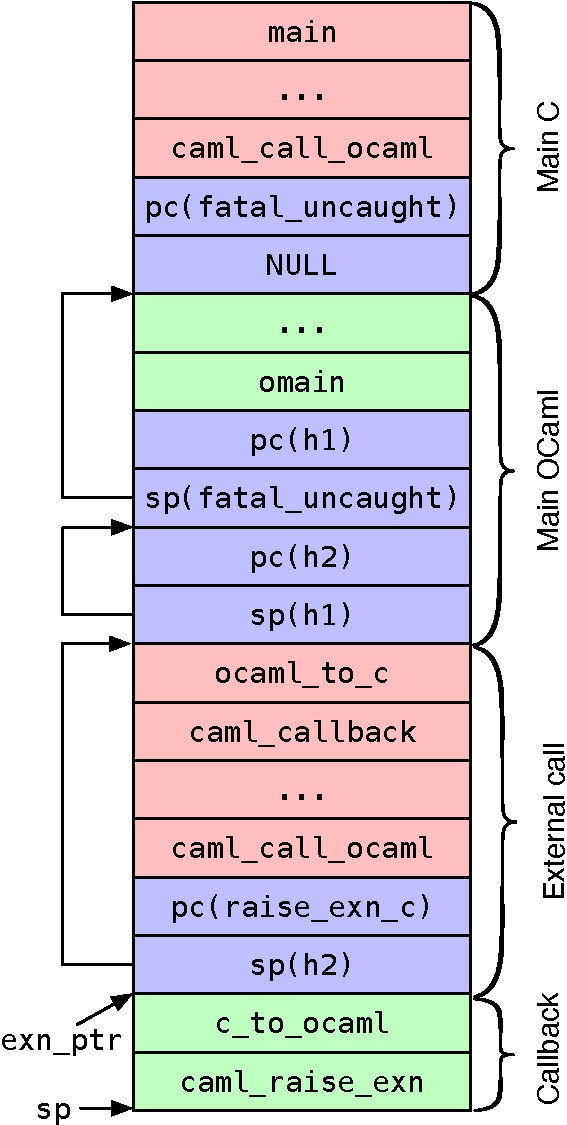
\includegraphics[scale=0.44]{figures/stock_stack}
  \subcaption{Stack layout before raise \texttt{E1}.}
  \label{fig:stock_stack}
\end{minipage}
%
\begin{minipage}{0.39\linewidth}
\begin{lstlisting}[language=c,basicstyle=\ttfamily\footnotesize]
#0  0x925dc in caml_raise_exn ()
#1  0x6fd3e in camlMeander__c_to_ocaml_83 () at meander.ml:5
#2  0x925a4 in caml_call_ocaml ()
#3  0x8a84a in caml_callback_exn (...) at callback.c:145
#4  caml_callback (...) at callback.c:199
#5  0x76e0a in ocaml_to_c (unit=1) at meander.c:5
#6  0x6fd77 in camlMeander__omain_88 () at meander.ml:10
#7  0x6fe92 in camlMeander__entry () at meander.ml:13
#8  0x6f719 in caml_program ()
#9  0x925a4 in caml_call_ocaml ()
#10 0x92e4c in caml_startup_common (...) at startup_nat.c:162
#11 0x92eab in caml_startup_exn (...) at startup_nat.c:167
#12 caml_startup (...) at startup_nat.c:172
#13 0x6f55c in main (...) at main.c:44
\end{lstlisting}
\vspace{-2mm}
\subcaption{\texttt{gdb} backtrace before raise \texttt{E1}.}
\label{code:gdb_backtrace}
\end{minipage}
\vspace{-2mm}
\caption{Program stack on stock OCaml.}
\vspace{-2mm}
\end{figure*}

The main challenge in implementing effect handlers in Multicore OCaml is
managing the program stack and preserving its desirable properties. In this
section, we provide an overview of the program stack and related mechanisms in
stock OCaml.

Consider the layout of the stock OCaml stack for the
program in Figures~\ref{code:meander_ml} and~\ref{code:meander_c}. The OCaml
main function |omain| installs two exception handlers |h1| and |h2| to handle
the exceptions |E1| and |E2|. |omain| calls the external C function |ocaml_to_c|,
which in turn calls back into the OCaml function |c_to_ocaml|, which raises the
exception |E1|. OCaml supports raising exceptions in C as well as throwing
exceptions across external calls. Hence, the exception |E1| gets caught in the
handler |h1|, and |omain| returns |42|. The layout of the stack in the native code
backend just before raising the exception in |c_to_ocaml| is illustrated in
Figure~\ref{fig:stock_stack}. Note that the stack grows downwards.

OCaml uses the same program stack as C, and hence the stack has
alternating sequences of C and OCaml frames. However, unlike C, OCaml does not
create pointers into OCaml frames. OCaml uses the hardware support for |call|
and |return| instructions for function calls and returns. OCaml does not
perform explicit stack overflow checks in code, and, just like C, relies on the
guard page at the end of the stack region to detect stack overflow. Stack
overflow is detected by a memory fault and a |Stack_overflow| exception is
raised to unwind the stack.

\subsection{External calls and callbacks}
\label{sec:external}

OCaml does not use the C calling convention. In particular, there are no
callee-saved registers in OCaml. In the |x86-64| backend, the OCaml runtime
makes use of two C callee-saved registers for supporting OCaml execution. The
register |r15| holds the \emph{allocation pointer} into the minor heap used for
bump pointer allocation, and |r14| holds a reference to the |Caml_state| table
of global variables used by the runtime. This makes external calls extremely
fast in OCaml. If the external function does not allocate in the OCaml heap,
then it can be called directly and no bookkeeping is necessary. For external
functions which allocate in the OCaml heap, the cached allocation pointer is
saved to |Caml_state| before the external call and it is restored on return.
Similarly, callbacks into OCaml are also cheap: these involve loading the
arguments in the right registers and calling the OCaml function. OCaml
callbacks are relatively common as the garbage collector (GC) finalisation
functions are executed as OCaml callbacks.

\subsection{Exception handlers}
\label{sec:exn_handlers}

The lack of callee-saved registers also makes exception handling fast as there
are no callee-saved registers to be restored when the exception handler runs.
Installing an exception handler simply pushes the program counter (|pc|) of the
handler and the current exception pointer (|exn_ptr| -- a field in
|Caml_state|) to the stack. After this, the current exception pointer is
updated to be the current stack pointer (|rsp|). This creates a linked-list of
exception handler frames on the stack as shown in Figure~\ref{fig:stock_stack}.
Raising an exception simply sets |rsp| to |exn_ptr|, loads the saved |exn_ptr|,
and jumps to the |pc| of the handler.

% Note |caml_call_ocaml| is |caml_start_program| in ocaml-multicore source

In order to forward exceptions across C frames, the C stub function
|caml_call_ocaml|, pushes an exception handler frame that forwards the
exception to the innermost OCaml exception handler (|raise_exn_c| in
Figure~\ref{fig:stock_stack}) or prints a fatal error (|fatal_uncaught|) if
there are no enclosing handlers. Exceptions are so cheap in OCaml that it is
common to use them for \emph{local} control flow.

\subsection{Stack unwinding}
\label{sec:unwind}

OCaml generates \emph{stack maps} in order to accurately identify roots on the
stack for assisting the GC. For every call point in the program, the OCaml
compiler emits the size of the frame and the set of all live registers in the
frame containing pointers into the heap. During a GC, the OCaml stack is walked
and the roots are marked skipping over the C frames.

OCaml also generates precise DWARF unwind information for OCaml, thanks to
which debuggers such as |gdb| and |lldb|, and profilers such as |perf| work
out-of-the-box. For example, for the program in Figures~\ref{code:meander_ml}
and~\ref{code:meander_c}, one could set a break point in |gdb| at
|caml_raise_exn| to get the backtrace in Figure~\ref{code:gdb_backtrace} which
corresponds to the stack in Figure~\ref{fig:stock_stack}.

The same backtrace can also be obtained by using \emph{frame pointers} instead
of DWARF unwind tables. OCaml allows compiling code with frame pointers, but
they are not enabled by default. OCaml stack tends to be deep with small frames
due to the pervasive use of recursive functions, not all of which are
tail-recursive. Hence, the addition of frame pointers can significantly
increase the size of the
stack\footnote{https://github.com/ocaml/ocaml/issues/5721\#issuecomment-472965549}.
Moreover, not using frame pointers saves two instructions in the function
prologue and epilogue, and makes an extra register (|rbp| on x86) available.
Note that the DWARF unwind information is complementary to the information used
by OCaml to walk the stack for GC.

\section{Refining the design}
\label{sec:refine}

In this section, we refine the effect handler design for the OCaml use case. The
primary motivation for adding effect handlers to OCaml is to support a non-local
control flow mechanism to implement asynchronous I/O in direct style, generators
and enable task parallelism. These use cases do not resume the continuations
more than once. Hence, our continuations are one-shot, and resuming the
continuation more than once raises |Invalid_argument| exception. It is
well-known that one-shot continuations can be implemented
efficiently~\cite{Bruggeman96}.

While OCaml permits throwing exceptions across C frames, we do not allow
effects to propagate across C frames as the C frames would become part of the
captured continuation. Managing C frames as part of the continuation is a
complex endeavour~\cite{Leijen17}, and we find that the complexity budget
outweighs the relatively fewer mechanisms enabled by this addition in our
setting.

The interaction of non-local control flow with systems programming is quite
subtle~\cite{TFP17}. Consider the following function that uses blocking I/O
functions from the OCaml standard library to copy data from the input channel
|ic| to the output channel |oc|:
\begin{lstlisting}
let rec copy ic oc =
  try output_string oc ((input_line ic) ^ "\n");
      copy ic oc
  with End_of_file -> close_in ic; close_out oc
	   | e -> close_in ic; close_out oc; raise e
\end{lstlisting}
The function |input_line| raises an |End_of_file| exception on reaching the end of
input, which is handled by the exception handler which closes the channels. The
|close_*| functions do nothing if the channel is already closed. The code is
written in a defensive style to handle other exceptional cases such as the
channels being closed externally. Both |input_line| and |output_string| raise
|Sys_error| exception if the channel is closed. In this case, the channels are
closed and the exception is reraised to communicate the exceptional behaviour
to the caller.

One of our goals (\S\ref{sec:req}) is to make this code transparently
asynchronous. We can define effects for performing the I/O operations and wrap
them up in functions with the same signature as the one from the standard
library:
\begin{lstlisting}
effect In_line : in_channel -> string
effect Out_str : out_channel -> string -> unit
let input_line ic = perform (In_line ic)
let output_string oc = perform (Out_str oc)
\end{lstlisting}

We can then use a top-level I/O handler similar to the introductory example
(\S\ref{sec:aio}) to discharge the I/O operations asynchronously and resumes
with the result. This handles value return cases, but what about the
exceptional cases |End_of_file| and |Sys_error|? We introduce a |discontinue|
primitive to resume a continuation by raising an exception. In this example, on
reaching the end of file, we would discontinue the continuation of the |copy|
function with |discontinue k End_of_file|, which raises the exception at
|input_line|, and the open channels will be closed.

Programs that use resources such as channels are usually written defensively
with the assumption that calling a function will return \emph{exactly once},
either normally or exceptionally. Since effect handlers in Multicore OCaml do
not ensure that all the effects are handled, if the function performs an effect
with no matching handler, then the function \emph{will not return at all}. To
remedy this, when such an effect bubbles up to the top-level, we discontinue the
continuation with an |Unhandled| exception so that the exception handlers may
run and clean up the resources.

\section{Semantics}
\label{sec:semantics}

\subsection{Static semantics}
\label{sec:static_semantics}

As mentioned earlier, effect handlers in Multicore OCaml do not guarantee
effect safety, but only guarantee type safety. Programs without matching effect
handlers are well-typed Multicore OCaml programs. As a result, our static
semantics is simpler than languages that ensure effect
safety~\cite{Hillerstrom20,Leijen14,Effekt,Frank,Biernacki19}. This is important for
backwards compatibility as our goal is to retrofit effect handlers to a
language with large legacy codebases. Programs that do not use effects remain
well-typed, and those that do compose well with those that don't.

The static semantics of effect handlers in OCaml is captured succinctly by its
API:
\begin{lstlisting}
type 'a eff = ..
type ('a,'b) continuation
val perform: 'a eff -> 'a
val continue: ('a,'b) continuation -> 'a -> 'b
val discontinue: ('a,'b) continuation -> exn -> 'b
(* Internal API *)
type 'a comp = unit -> 'a
type ('a,'b) handler =
{retc: 'a -> 'b;
 effc: 'c.'c eff -> ('c,'b) continuation -> 'b; }
val match_with: 'a comp -> ('a,'b) handler -> 'b
\end{lstlisting}
We introduce an extensible variant type~\cite{ExtVariants} |'a eff| of effect
values, which when performed using the |perform| primitive returns a |'a|
value. Constructors for the value of type |'a eff| are declared using the
effect declarations. For example, the declaration |effect E : string -> int|
is syntactic sugar for adding a new constructor to the variant type
|type _ eff += E : string -> int eff|. We introduce the type
|('a,'b) continuation| of delimited continuations which expect a |'a| value for
resumption and return |'b| value. The continuations may be continued with a
suitably typed value or discontinued with an exception.

For handling the effects, our implementation extends OCaml's |match ... with|
syntax with effect patterns. The expression
\begin{lstlisting}
match e with
| None -> false | Some b -> b
| effect (E s) k1 -> e1 | effect (F f) k2 -> e2
\end{lstlisting}
\noindent is translated to the equivalent of
\begin{lstlisting}
match_with (fun () -> e)
{ retc = (function None -> false | Some b -> b);
  effc = (function
  | (E s) -> (fun k1 -> e1)
  | (F f) -> (fun k2 -> e2)
  | e -> (fun k -> match perform e with
          | v -> continue k v
          | exception e -> discontinue k e)); }
\end{lstlisting}
For the sake of exposition, we introduce a |('a,'b) handler| type. This handler
handles a |'a comp| that returns a |'a| value, and itself returns a |'b| value.
The handler has a return case of type |'a -> 'b|. The effect case |effc|
handles effects of type |'c eff| with |('c,'b) continuation| and returns a
value of type |'b|. The last case in |effc| \emph{reperforms} any unmatched
effect to the outer handler and returns the value and exceptions back to the
original performer. In the implementation, reperfom is implemented as a
primitive to avoid executing code on the resumption path.

\begin{figure*}
\begin{minipage}{\linewidth}
  \begin{minipage}[t]{0.49\linewidth}
  \begin{smathpar}
  \begin{array}{rrcl}
    \text{Constants} & n & \coloneqq & ℤ \\
    \text{Abstractions} & \Lambda & \coloneqq & \lambda^o \mid \lambda^c \\
    \text{Expressions} & e & \coloneqq & n \mid x \mid e ~e \mid  \lam{x}{e} \mid e \odot e \mid \throw{l}{e} \\
                       &   & \mid      & \handle{e}{h} \mid \perform{l}{e} \\
    \text{Handlers} & h & \coloneqq & \{\caseval{x}{e}\} \mid \{\caseexn{l}{x}{e}\} \uplus h \\
                   &   & \mid & \{\caseeff{l}{x}{k}{e}\} \uplus h \\
    \text{Values} & v & \coloneqq & n \mid k \mid \clos{x}{e}{\env} \mid \effval{l}{k} \mid \exnval{l} \\
    \text{Frames} & r & \coloneqq & \farg{e}{\env} \mid \ffun{v} \mid \faritha{\odot}{e}{\env} \mid \farithb{\odot}{ℕ} \\
    \text{Environments} & \env & \coloneqq & \emptyset \mid \envext{\env}{x}{v} \\
  \end{array}
  \end{smathpar}
  \end{minipage}
  \begin{minipage}[t]{0.49\linewidth}
  \begin{smathpar}
  \begin{array}{rrcl}
    \text{Handler Closures} & \hc & \coloneqq & (h,\env) \\
    \text{Frame List} & \fl & \coloneqq & [] \mid r :: \fl \\
    \text{Fibers} & \fiber & \coloneqq & (\fl, \hc) \\
    \text{Continuations} & k & \coloneqq & [] \mid \fiber \kcons k \\
    \text{C stacks} & \cstack & \coloneqq & \cstacka{\fl}{\ostack}\\
    \text{OCaml stacks} & \ostack & \coloneqq & \ostacka{k}{\cstack} \mid \ostackemp \\
    \text{Stacks} & \stack & \coloneqq & \cstack \mid \ostack \\
    \text{Terms} & \term & \coloneqq & e \mid v \\
    \text{Configurations} & \config & \coloneqq & \configa{\tau}{\env}{\stack}
  \end{array}
  \end{smathpar}
	\end{minipage}
  \subcaption{Syntax of expressions and configurations}
  \label{sem:syntax}
\end{minipage}
%
\begin{minipage}{\linewidth}
	\begin{smathpar}
		\begin{array}{cc}
			\textsc{StepC} ~
			\inferrule{(\term, \env, \fl, \ostack) \cstep \config}
								{\configa{\term}{\env}{\cstacka{\fl}{\ostack}} \step \config} &
			\textsc{StepO} ~
			\inferrule{(\term, \env, k, \cstack) \ostep \config}
								{\configa{\term}{\env}{\ostacka{k}{\cstack}} \step \config}
		\end{array}
	\end{smathpar}
	\subcaption{Top-level reductions}
	\label{sem:toplevel}
\end{minipage}
%
\begin{minipage}{\linewidth}
  \begin{smathpar}
    \begin{array}{rrcl}
      \textsc{Var}     & (x,\env, \fl) & \rightsquigarrow
                       & (\env(x), \env, \fl) \\
      \textsc{Arith1}  & (e_1 \odot e_2, \env, \fl) & \rightsquigarrow
                       & (e_1,\env, \faritha{\odot}{e_2}{\env}::\fl) \\
      \textsc{Arith2}  & (n_1, \_, \faritha{\odot}{e_2}{\env}::\fl) & \rightsquigarrow
                       & (e_2, \env, \farithb{\odot}{n_1}::\fl) \\
      \textsc{Arith3}  & (n_2, \env, \farithb{\odot}{n_1}::\fl) & \rightsquigarrow
                       & (\llbracket n_1 \odot n_2 \rrbracket, \env, \fl) \\
      \textsc{App1}    & (e_1 ~e_2, \env, \fl) & \rightsquigarrow
                       & (e_1, \env, \farg{e_2}{\env}::\fl) \\
      \textsc{App2}    & (\lam{x}{e}, \env, \fl) & \rightsquigarrow
                       & (\clos{x}{e}{\env}, \env, \fl) \\
      \textsc{App3}    & (\clos{x}{e_1}{\env_1}, \_, \farg{e_2}{\env_2}::\fl) & \rightsquigarrow
                       & (e_2, \env_2, \ffun{\clos{x}{e_1}{\env_1}}::\fl) \\
      \textsc{Resume1} & (k,\_,\farg{e_1}{\env_1}::\farg{e_2}{\env_2}::\fl) & \rightsquigarrow
                       & (e_1, \env_1, \ffun{k}::\farg{e_2}{\env_2}::\fl) \\
      \textsc{Resume2} & (\clos{x}{e_1}{\env_1}, \_, \ffun{k}::\farg{e_2}{\env_2}::\fl) & \rightsquigarrow
                       & (e_2, \env_2, \ffun{k}::\ffun{\clos{x}{e_1}{\env_1}}::\fl) \\
      \textsc{Perform} & (\perform{l}{e}, \env, \fl) & \rightsquigarrow
                       & (e, \env, \ffun{\effval{l}{[[],(\{\caseval{x}{x}\},\emptyset)]}}::\fl) \\
      \textsc{Raise}   & (\throw{l}{e}, \env, \fl) & \rightsquigarrow
                       & (e, \env, \ffun{\exnval{l}}::\fl)
    \end{array}
  \end{smathpar}
  \subcaption{Administrative Reductions -- $(\term, \env, \fl) \rightsquigarrow (\tau, \env, \fl)$.}
  \label{sem:step}
\end{minipage}
%
\begin{minipage}{\linewidth}
  \begin{smathpar}
    \begin{array}{rrcll}
      \textsc{AdminC}   & (\term,\env,\fl,\ostack) & \cstep
                        & \configa{\term'}{\env'}{\cstacka{\fl'}{\ostack}}
                        & \text{if } (\term,\env,\fl) \rightsquigarrow (\term',\env',\fl') \\
      \textsc{RetToO}   & (v,\env,[],\ostacka{k}{\cstack}) & \cstep
                        & \configa{v}{\env}{\ostacka{k}{\cstack}} \\
      \textsc{CallC}    & (v, \_, \cclos{x}{e}{\env}::\fl, \ostack) & \cstep
                        & \configa{e}{\envext{\env}{x}{v}}{\cstacka{\fl}{\ostack}} \\
      \textsc{Callback} & (v, \_, \oclos{x}{e}{\env}::\fl, \ostack) & \cstep
                        & \configa{e}{\envext{\env}{x}{v}}{\ostacka{k}{\cstacka{\fl}{\ostack}}}
                        & \text{if } k = [[],(\{\caseval{x}{x}\},\emptyset)] \\
      \textsc{ExnFwdO}  & (v, \env, \ffun{\exnval{l}}::\_, \ostacka{(\fl,\hc) \kcons k}{\cstack}) & \cstep
                        & \configa{v}{\env}{\ostacka{(\ffun{\exnval{l}}::\fl,\hc) \kcons k}{\cstack}}
    \end{array}
  \end{smathpar}
  \subcaption{C Reductions -- $(\term, \env, \fl, \ostack) \cstep \config$.}
  \label{sem:cstep}
\end{minipage}
%
\begin{minipage}{\linewidth}
  \begin{smathpar}
    \begin{array}{rrcll}
      \textsc{AdminO}   & (\term,\env,(\fl,\hc) \kcons k,\cstack) & \ostep
                        & \configa{\term'}{\env'}{\ostacka{(\fl',\hc) \kcons k}{\cstack}}
                        & \text{if } (\term,\env,\fl) \rightsquigarrow (\term',\env',\fl') \\
      \textsc{RetToC}   & (v, \_, [([],(h,\emptyset))], \cstack) & \ostep
                        & \configa{v}{\env}{\cstack}
                        & \text{if } h = \{\caseval{x}{x}\} \\
      \textsc{RetFib} & (v, \_, ([],(h,\env)) \kcons k, \cstack) & \ostep
                        & \configa{e}{\envext{\env}{x}{v}}{\ostacka{k}{\cstack}}
                        & \text{if } \{\caseval{x}{e}\} \in h \\
      \textsc{CallO}    & (v, \_, (\oclos{x}{e}{\env}::\fl,\hc) \kcons k, \cstack) & \ostep
                        & \configa{e}{\envext{\env}{x}{v}}{\ostacka{(\fl,\hc) \kcons k}{\cstack}} \\
      \textsc{ExtCall}  & (v, \_, (\cclos{x}{e}{\env}::\fl,\hc) \kcons k, \cstack) & \ostep
                        & \configa{e}{\envext{\env}{x}{v}}{\cstacka{[]}{\ostacka{(\fl,\hc) \kcons k}{\cstack}}} \\
      \textsc{Resume}   & (v, \_, (\ffun{k}::\ffun{\oclos{x}{e}{\env}}::\fl,\hc) \kcons k, \cstack) & \ostep
                        & \configa{e}{\envext{\env}{x}{v}}{\ostacka{k ~@~ ((\fl,\hc) \kcons k')}{\cstack}} \\
      \textsc{Handle}   & (\handle{e}{h}, \env, k, \cstack) & \ostep
                        & \configa{e}{\env}{\ostacka{([],(h,\env)) \kcons k}{\cstack}} \\
      \textsc{EffUnHn}  & (v, \_, [\ffun{\effval{l}{k}}::\fl,(h,\env)], \cstack) & \ostep
                        & \configa{e}{\emptyset}{\ostacka{k ~@~ [(\fl,(h,\env))]}{\cstack}}
                        & \text{if } \{\caseeff{l}{\_}{\_}{\_}\} \notin h \\
                  & & & & \text{and } {e = \throw{\textsf{unhandled}}{0}} \\
      \textsc{EffHn}    & (v, \_, (\ffun{\effval{l}{k}}::\fl,(h,\env)) \kcons k', \cstack) & \ostep
                        & \configa{e}{\env[r \mapsto k''][x \mapsto v]}{\ostacka{k'}{\cstack}}
                        & \text{if } \{\caseeff{l}{x}{r}{e}\} \in h \\
                  & & & & \text{and } k'' = k ~@~ [(\fl,(h,\env))] \\
      \textsc{EffFwd}   & (v, \env', (\ffun{\effval{l}{k}}::\fl,(h,\env)) \kcons (\fl',\hc') \kcons k', \cstack) & \ostep
                        & \configa{v}{\env'}{\ostacka{(\ffun{\effval{l}{k''}}::\fl',\hc') \kcons k'}{\cstack}}
                        & \text{if } \{\caseeff{l}{\_}{\_}{\_}\} \notin h \\
                  & & & & \text{and } k'' = k ~@~ [(\fl,(h,\env))] \\
      \textsc{ExFwdC}   & (v, \env, [\ffun{\exnval{l}}::\_,(h,\_)], \cstacka{\fl'}{\ostack}) & \ostep
                        & \configa{v}{\env}{\cstacka{\ffun{\exnval{l}}::\fl'}{\ostack}}
                        & \text{if } \{\caseexn{l}{\_}{\_}\} \notin h \\
      \textsc{ExHn}     & (v, \_, (\ffun{\exnval{l}}::\_,(h,\env)) \kcons k', \cstack) & \ostep
                        & \configa{e}{\envext{\env}{x}{v}}{\ostacka{k'}{\cstack}}
                        & \text{if } \{\caseexn{l}{x}{e}\} \in h \\
      \textsc{ExFwdFib} & (v, \env, (\ffun{\exnval{l}}::\_,(h,\_)) \kcons (\fl',\hc') \kcons k', \cstack) & \ostep
                        & \configa{v}{\env}{\ostacka{(\ffun{\exnval{l}}::\fl',\hc') \kcons k'}{\cstack}}
                        & \text{if } \{\caseexn{l}{\_}{\_}\} \notin h \\
    \end{array}
  \end{smathpar}
  \subcaption{OCaml Reductions -- $(\term, \env, k, \cstack) \ostep \config$.}
  \label{sem:ostep}
\end{minipage}
\caption{Operational semantics of Multicore OCaml effect handlers.}
\end{figure*}

\subsection{Dynamic semantics}

We present an operational semantics for a core language of effect handlers that
faithfully captures the semantics of the Multicore OCaml implementation.

\textbf{\textit{Syntax.}} Our expressions (Figure~\ref{sem:syntax}) consists of
integer constants ($n$), variables ($x$), abstraction ($\lam{x}{x}$),
application ($e~e$), arithmetic expressions ($e \odot e$) where $\odot$ ranges
over $\{+,-,*,/\}$, raising exceptions ($\throw{l}{e}$), performing effects
($\perform{l}{e}$), and handling effects ($\handle{e}{h}$). Abstractions come
in two forms: OCaml abstractions ($\lambda^o$) and C abstractions
($\lambda^c$). The handler consists of a return case ($\caseval{x}{e}$), zero
or more exception cases ($\caseexn{l}{x}{e}$) with label $l$, parameter $x$ and
body $e$, and zero or more effect cases ($\caseeff{l}{x}{k}{e}$) with label
$l$, parameter $x$, continuation $k$ and body $e$.

The operational semantics is an extension of a CEK machine
semantics~\cite{Felleisen86} for effect handlers, following the abstract
machine semantics of Hillerstrom et al.~\cite{Hillerstrom20}. The key
difference from Hillerstrom et al. is that our stacks are composed of
alternating sequence of OCaml and C stack segments. The program state is
captured as configuration $\config \coloneqq \configa{\tau}{\env}{\stack}$ with
the current term $\tau$ under evaluation, its environment $\env$ and the
current stack $\stack$. The term is either an expression $e$ or a value $v$.
The value are integer constants $n$, continuations $k$, closure
$\clos{x}{e}{\env}$, effect being performed ($\effval{l}{k}$) and exception
being raised ($\exnval{l}$). The environment is a map from variables to values.

The stack $\stack$ is either a C stack ($\cstack$) or an OCaml stack
($\ostack$). Every C stack $\cstacka{\fl}{\ostack}$ consists of a list of
frames $\fl$, and the OCaml stack $\ostack$ under it. Every OCaml stack is
either empty $\ostackemp$ or non-empty $\ostacka{k}{\cstack}$ with the C stack
$\cstack$ under it. Thus, the program stack is an alternating sequence of C and
OCaml stacks terminating with an empty OCaml stack $\ostackemp$. The frame list
$\fl$ is composed of individual frames $r$, which is one of an argument frame
$\farg{e}{\env}$ with the expression $e$ at the argument position of an
application with its environment $\env$, a function frame $\ffun{v}$ with the
value $v$ at the function position of an application, and frames for evaluating
the arguments of an arithmetic expression.

Continuations $k$ are either empty $[]$ or non-empty sequence of \emph{fibers}.
A fiber $\fiber \coloneqq (\fl,\hc)$ is a list of frames $\fl$ and a handler
closure $\hc \coloneqq (h,\env)$, which is a pair of handler $h$ and its
environment $\env$.

\textbf{\textit{Top-level reductions.}} The initial configuration for an expression
$e$ is $\configa{e}{\emptyset}{\cstacka{[]}{\bullet}}$, where the environment
and the stack are empty. The top-level reductions (Figure ~\ref{sem:toplevel})
can be performed by either by taking a C step $\cstep$ or an OCaml step
$\ostep$.

\textbf{\textit{C reductions.}} We can take a C step (Figure~\ref{sem:cstep}) by
taking an administrative reduction step $\rightsquigarrow$. The administrative
reductions are common to both C and OCaml. The rules \textsc{Var},
\textsc{Arith1}, \textsc{Arith2}, \textsc{App1}, \textsc{App2} and
\textsc{App3} are standard. \textsc{Arith3} performs the arithmetic operation
on the integers ($\llbracket n_1 \odot n_2 \rrbracket$). \textsc{Raise} pushes
an function frame with exception value to indicate that an exception is being
raised. Similarly, \textsc{Perform} pushes a function frame with an effect
value with an empty continuation $[[],(\{\caseval{x}{x}\},\emptyset)]$ with no
captured frames and an empty handler with an identity return case alone. We
shall return to \textsc{Resume1} and \textsc{Resume2} later.

Continuing with the rest of the C reduction steps, \textsc{CallC} captures the
behaviour of calling a C function. Since the program is currently executing C,
we can perform the call on the current stack. In case the abstraction is an
OCaml abstraction (\textsc{Callback}), we create an OCaml stack with the C
stack as its tail, with the current continuation being empty. This captures the
behaviour of calling back into OCaml from C. \textsc{RetToO} returns a value to
the enclosing OCaml stack. \textsc{ExnFwdO} forwards a raised exception to the
enclosing OCaml stack, unwinding the rest of the frames. This captures the
semantics of raising OCaml exceptions from C.

\textbf{\textit{OCaml reductions.}} In OCaml (Figure~\ref{sem:ostep}), reductions
always occur on the top-most fiber in the current stack. \textsc{AdminO}
performs administrative reductions. \textsc{CallO} evaluates an OCaml function
on the current stack. \textsc{ExtCall} captures the behaviour of external
calls, which are evaluated on an empty C stack. \textsc{RetToC} returns a value
to the enclosing C stack. In this case, we have exactly one fiber on the stack,
and this was created in the rule \textsc{Callback}, whose handler has identity
return case alone and the environment is empty. \textsc{RetFib} returns value
from a fiber to the previous one, evaluating the body of the return case.

The rule \textsc{Handle} installs a handler by pushing a fiber with no frames
and the given handler. The rule \textsc{ExHn} handles an exception, if the
current handler has a matching exception case, unwinding the current fiber. The
rule \textsc{ExFwdC} forwards the exception to C. Here, there is exactly one
fiber on the current stack, and the handler does not have a matching exception
case, which we know is the case (see \textsc{Callback} rule). The rule
\textsc{ExFwdFib} forwards the exception to the next fiber if the current
handler does not handle it.

The rule \textsc{EffHn} captures the handling of effects when the current
handler has a matching effect case. We evaluate the body of the matching case,
and bind the continuation parameter |r| to the captured continuation. Observe
that the captured continuation |k''| includes the current handler. Intuitively,
the handler wraps around captured continuation. This gives Multicore OCaml
effect handlers deep handler semantics~\cite{Hillerstrom20}. \textsc{EffFwd} forwards the
effect to the outer fiber, and extends the captured continuation |k''| in the
process. Recall that we do not capture C frames as part of a continuation. To
this end, \textsc{EffUnHn} models unhandled effect. If the effect bubbles up to
the top fiber, which we know does not have an effect case (see
\textsc{Callback} rule), we raise \textsc{unhandled} exception at the point
where the corresponding effect was performed. This is achieved by appending the
captured continuation to the front of the current continuation.

Observe that |continue| and |discontinue| are not part of the expressions. They
are encoded as follows: $\textsf{continue} ~k ~e = (k ~(\olam{x}{x})) ~e$ and
$\textsf{discontinue} ~k ~l ~e = (k ~(\olam{x}{\throw{l}{x}})) ~e$.
Intuitively, resuming a continuation in both the cases involves evaluating the
appropriate abstraction on top of the continuation. We perform the
administrative reductions \textsc{Resume1} and \textsc{Resume2} to evaluate the
arguments to |continue| and |discontinue|. The rule \textsc{Resume} appends the
given continuation to the front of the current continuation, and evaluates the
body of the closure.

The traces of example programs are included in the supplementary material along
with an executable version of the semantics implemented in OCaml.

\section{Implementation}
\label{sec:impl}

In this section, we present the implementation details of effect handlers in
Multicore OCaml. Multicore OCaml currently only supports the x86-64 backend on
Linux, but our design does not preclude other backends. We assume x86-64
architecture in the sequel.

\subsection{Exceptions}

The implementation follows the operational semantics, but has a few key
representational differences. Unlike the operational semantics, handlers with
just exception patterns (exception handlers) are implemented differently than
effect handlers. As mentioned in \S~\ref{sec:exn_handlers}, exceptions are
pervasive in OCaml and are so cheap that they are used for local control flow.
Hence, we retain the linked exception handler frame implementation of stock
OCaml exception handlers in Multicore OCaml for performance backwards
compatibility. This differs from other research languages with effect
handlers~\cite{Hillerstrom20,Frank,Eff}, which implement exceptions using
effects (by ignoring the continuation argument in the handler).

\subsection{Heap-allocated fibers}

\begin{figure*}
\begin{minipage}{0.35\linewidth}
  \centering
  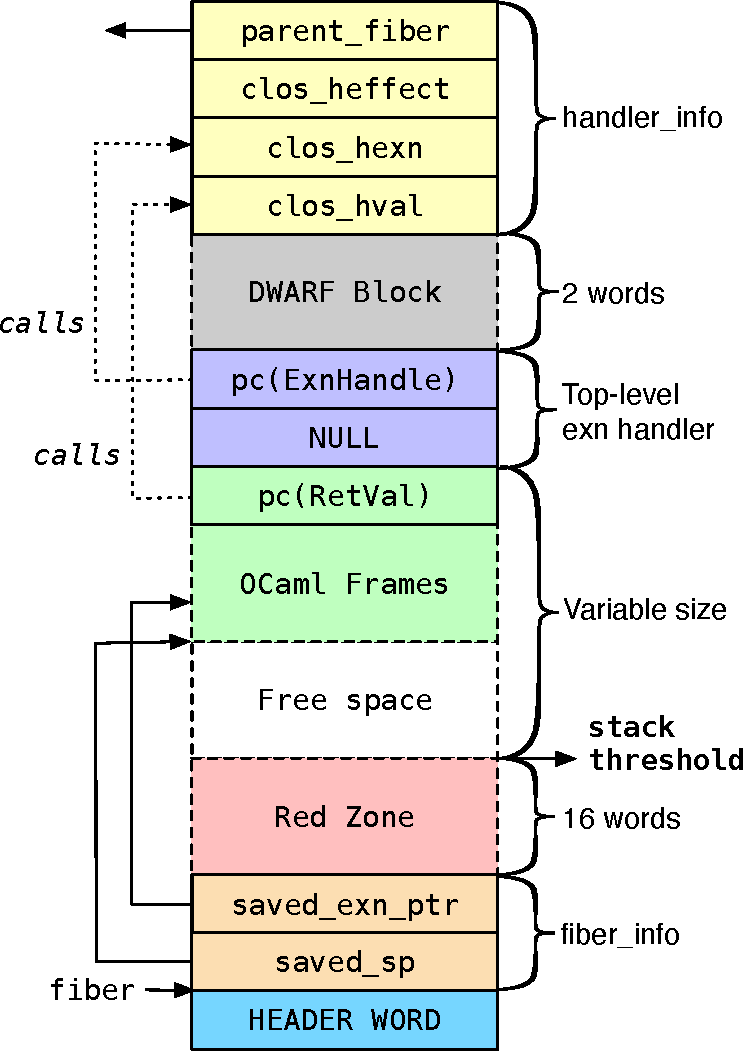
\includegraphics[scale=0.45]{figures/fiber}
  \subcaption{Fiber layout}
  \label{fig:fiber}
\end{minipage}
\begin{minipage}{0.64\linewidth}
  \begin{minipage}{\linewidth}
    \centering
    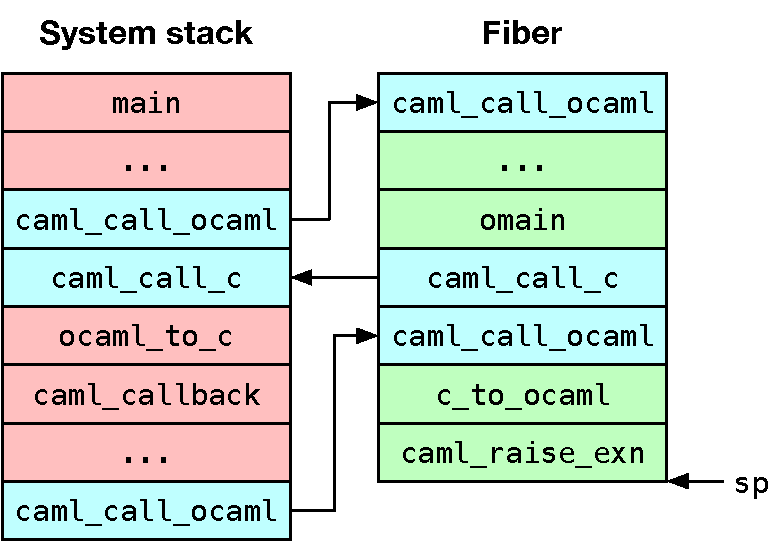
\includegraphics[scale=0.4]{figures/multicore_stack}
    \subcaption{Stack layout for \texttt{meander} example from \S\ref{sec:stack}.}
    \label{fig:mcstack}
    \vspace{2mm}
  \end{minipage}
  %
  \begin{minipage}{0.55\linewidth}
    \begin{lstlisting}
effect E : unit
effect F : unit;;
match (* comp_e *)
  match (* comp_f *)
    (*p1*) perform E (*p3*)
	with | v -> v | effect F kf -> ()
with | v -> v
		 | effect E ke -> (*p2*) continue ke ()
    \end{lstlisting}
		\subcaption{Constructing continuation objects}
		\label{code:effimpl}
  \end{minipage}
  %
  \begin{minipage}{0.44\linewidth}
    \centering
    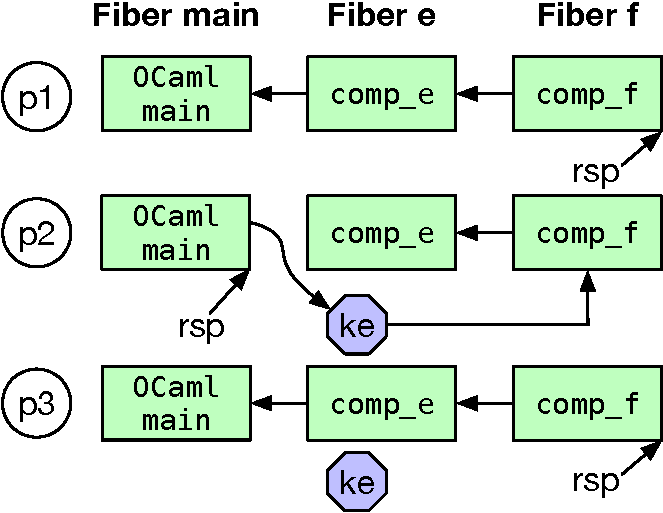
\includegraphics[scale=0.42]{figures/fiber_handler}
		\subcaption{Program state for code in~\ref{code:effimpl}}
    \label{fig:fiber_handler}
  \end{minipage}
\end{minipage}
\vspace{-2mm}
\caption{Layout of Multicore OCaml effect handlers.}
\vspace{-3mm}
\end{figure*}

In the operational semantics, the continuations may be resumed more than once.
Captured continuations are copies of the original fibers and resuming the
continuation copies the fibers and leaves the continuation as it is. In our use
cases, continuations will be resumed at-most once, and copying fibers is
unnecessary and inefficient. Instead, Multicore OCaml optimises fibers for
one-shot continuations.

Fibers are allocated on the heap using |malloc| and are |free|d when no longer
necessary. We do not use a \emph{stack cache} of recently freed stacks for
speeding up fiber allocation~\cite{Farvardin20}. In our experiments, we
observed that directly using |mimalloc|~\cite{Leijen19} outperforms a stack
cache.

Figure~\ref{fig:fiber} shows the layout of a fiber in Multicore
OCaml. At the bottom of the stack, we have the |handler_info|, which contains
the pointer to parent fiber, and the closures for the value, exception and
effect cases. The closures are created by the translation described in
\S\ref{sec:static_semantics}; Multicore OCaml supports exception patterns in
addition to effect patterns in the same handler. This is followed by a context
block needed for DWARF and GC bookkeeping with callbacks. Then, there is a
top-level handler that invokes the exception handler |clos_hexn| after
switching to the parent fiber. This is followed by the |pc| of the code that
invokes the value handler |clos_hval| after switching to the parent stack. The
stack is laid out such that when the computation in the handler returns,
control goes to the value handler.

We have the variable-sized area for the OCaml frames next. Since we want the
fibers to be as small as possible, this area is initially 16 words in length.
When the stack pointer |rsp| becomes less than the stack threshold (maintained
in the |Caml_state| table), the stack is said to have overflown. On stack
overflow, we copy the whole fiber to a new area with double the size. In
Multicore OCaml, we introduce stack overflow checks into the function prologue
of OCaml functions. In our evaluation of real world OCaml programs, we observed
that most function calls are to leaf functions with small frame size. In order
to take advantage of this fact, we introduce a small red zone at the top of the
stack. The compiler elides the stack overflow check for leaf functions whose
frame size is less than the size of the red zone.

Finally, we have the saved exception pointer, which points to the top-most
exception frame, and the saved stack pointer, which points to the top of the
stack. Switching between fibers only involves saving the exception and the
stack pointer of the current stack and loading the same on the target stack.
Since OCaml does not generate pointers into the stack, the two |fiber_info|
fields are the only ones that need to be updated when fibers are moved.

\subsection{External calls and callbacks}

Since C functions do not have stack overflow checks, we have to execute the
external calls in the system stack. Calling a C function from OCaml involves
saving the stack pointer in the current fiber, saving the allocation pointer in
the |Caml_state|, updating |rsp| to the top of system stack (maintained in
|Caml_state|), and calling the C function. The actions are reversed when
returning from the external call. For C functions that take arguments on the
stack, the arguments must be copied to the C stack from the OCaml stack where
they are laid out. In the vast majority of external calls, we perform only a
few additional instructions over stock OCaml.

When we first enter OCaml from C, a new fiber is allocated for the main OCaml
stack. Since callbacks may be frequent in OCaml programs that use finalisers,
we run the callbacks on the same fiber as the current one. For example, the
layout of the Multicore OCaml stack at |caml_raise_exn| in the |meander|
example from \S\ref{sec:stack} is shown in Figure~\ref{fig:mcstack}. The
functions |caml_call_c| and |caml_call_ocaml| switch the stacks, and hence are
shown in both the system stack and the fiber. Since we are reusing the fiber
for the callback, care must be taken to save and restore the |handler_info|
before calling and after returning from |c_to_ocaml| function, respectively.
Thanks to the fiber representation, external calls and callbacks remain
competitive with stock OCaml.

\subsection{Effect handlers}
\label{sec:effimpl}

In order to illustrate the implementation of handling effects, consider the
example presented in Figure~\ref{code:effimpl}. The layout of the program state
as the program executes is captured in Figure~\ref{fig:fiber_handler}. The code
performs |E| which is handled in the outer-most handler, and is immediately
resumed. The arrows between the fibers are parent pointers. At position |p1|,
|rsp| is at the top of the fiber |f|.

When the effect |E| performed, we allocate a continuation object |ke| in the
heap that points to the current fiber |f|, set fiber |f|'s parent pointer to
|NULL|, and evaluate the continuation closure |clos_heffect| on the parent
fiber |e| with the effect |E| and the continuation |ke| as arguments. Since the
first handler does not handle effect |E|, the effect is \emph{reperformed}
(\S\ref{sec:static_semantics}) by appending the fiber |e| to the tail of
continuation |ke|, set fiber |e|'s parent pointer to |NULL|, and evaluate the
current continuation closure on the parent fiber |main| with |E| and |ke| as
arguments, which handles |E| (position |p2|). Thus, \emph{continuations are
captured without copying frames}. Since every handler closure is evaluated
until a matching one is found, the time taken to handle an effect is linear in
the number of handlers. We observe that the handler stack is shallow in real
programs.

When the continuation is resumed, we overwrite the value of |ke| to |NULL| to
enforce at-most once semantics. Resuming a continuation involves traversing the
linked-list of fibers and making the last fiber point to the current fiber.
Just as in the operational semantics, the implementation invokes the
appropriate closure to either |continue| or |discontinue| the continuation
(position |p3|). We perform standard tail-call optimisation so that resumptions
at tail positions do not build up stack.

\subsection{Stack unwinding}

The challenge with DWARF stack unwinding is to make it aware of the
non-contiguous stacks. While the complete details of DWARF stack unwinding is
beyond the scope of the paper, it is beneficial to know how DWARF unwind tables
are constructed in order to appreciate our solution. We refer the interested
reader to Bastian et al.~\cite{Bastian19} for a good overview of DWARF stack
unwinding.

Logically, DWARF call-frame information maintains a large table which records
for every machine instruction where the return address and callee-saved
registers are stored. To avoid reifying this large table, DWARF directives
represent the table using a compact bytecode representation. This representation
is interpreted on demand for building the stack unwind table. Within each
function, DWARF maintains a \emph{canonical frame address} (CFA) and is
traditionally the stack pointer before entering this function. Hence, on x86-64,
where the return address is pushed on the stack on call, the return address is
at |CFA - 8|.

One challenge is to encode in DWARF directives the CFA when stacks are switched
at effect handlers, callbacks and external calls. When starting to run on a new
fiber, we insert DWARF bytecode to follow the |parent_fiber| pointer and
dereference the |saved_sp| to get the CFA (|saved_sp + 8|). During callbacks
into OCaml, we save the current system stack pointer in the |context block| in
Figure~\ref{fig:fiber} to identify the CFA in the C stack. DWARF unwinding for
external calls is implemented by following a link to the current OCaml stack
pointer. With these changes, we get the same backtrace for the \texttt{meander}
program from \S\ref{sec:unwind}, modulo runtime system functions due to effect
handlers.

We have utilized a DWARF verification tool~\cite{Bastian19} with extensions to
handle PIE and additional DWARF primitives to flag possible errors in the hand
written DWARF directives where we have altered the OCaml assembler to implement
effects. In three places additional manual verification was required; two were
where the stack is intentionally switched between fibers and one was where the
return to the parent stack on child stack completion could not track stack
resizes and intermediate effect handler frames.

Even with correct DWARF unwind information, using DWARF to record call stack
information in |perf| only captures the call stack of the current fiber in
Multicore OCaml. Since stack unwinding using DWARF is slow due to bytecode
interpretation overhead, |perf| dumps the (user) call stack when
sampled~\cite{Bastian19}. This only includes the frames from the current fiber.
This is a limitation of |perf| and not of our stack layout.

\subsection{Garbage collection}

Recall that OCaml programs are written with the expectation that function calls
return exactly once (\S\ref{sec:refine}). Consider the scenario when a
continuation is neither continued nor discontinued. Since fibers are
|malloc|ed and are |free|d when the computation being handled returns a value
or raises an exception, not resuming continuations leaks memory. In addition,
unresumed continuations may also leak other resource such as open file
descriptors.

We consider well-behaved Multicore OCaml programs to resume their continuations
\emph{exactly once}. This can be enforced by installing a finaliser on every
captured continuation that |discontinue|s the continuation during finalisation
and ignores the result:
\begin{lstlisting}
Gc.finalise (fun k ->
  try ignore (discontinue k Unwind) with _ -> ()) k
\end{lstlisting}
Multicore OCaml does not enforce this behaviour in order to avoid installing an
effect handler every time a continuation is captured.

For stack walking during GC, the only change necessary was to make the runtime
aware of fiber layout and how to follow the parent pointers. The stack map
generation and scanning each frame for roots remains the same. Sivaramakrishnan
et al.~\cite{Sivaramakrishnan20} present the challenges and solutions for
integrating fibers with the concurrent mark-and-sweep GC of Multicore OCaml.

\section{Evaluation}
\label{sec:eval}

In this section, we evaluate the performance of Multicore OCaml effect handlers
against the performance requirements set in \S\ref{sec:req}. Multicore OCaml is
an extension of 4.10.0 OCaml compiler with support for shared memory
parallelism and effect handlers. These results were obtained on 2-socket,
Intel\textregistered Xeon\textregistered Gold 5120 x86-64 server, with 28
physical cores (14 cores on each socket), and 2 hardware threads per core. Each
core runs at 2.20GHz and has 32 KB of L1 data cache, 32 KB of L1 instruction
cache and 1MB of L2 cache. The cores on a socket share a 19.25 MB L3 cache. The
server has 64GB of main memory and runs Ubuntu 18.04.

\vspace{-3mm}
\subsection{No effects benchmarks}

In this section, we measure the impact of the addition of effect handlers on
code that does not use effect handlers. Our macro benchmark suite consists of
54 real OCaml workloads including verification tools (|Coq|, |Cubicle|,
|AltErgo|), parsers (|menhir|, |yojson|), storage engines (|irmin|), utilities
(|cpdf|, |decompress|), bioinformatics (|fasta|, |knucleotide|, |revcomp2|,
|regexredux2|), numerical analysis (|grammatrix|, |LU_decomposition|) and
simulations (|nbody|, |game_of_life|). In addition to Stock (|stock|) and
Multicore OCaml (|MC|), we also ran the benchmarks on Multicore OCaml with no
red zone (|MC+RedZone0|) in the fiber (all OCaml functions will have stack
overflow check) and a red zone size of 32 words (|MC+RedZone32|). Recall that
the default red zone size in Multicore OCaml is 16 words.

The complete results are presented in the supplementary material, which we
summarise here. On average (geometric mean of the normalized values against
|stock| as the baseline), the multicore variants were \textbf{less than 1\%
slower}. The outliers (on either ends) were due to the difference in the
allocator and the GC between stock and Multicore OCaml. The biggest impact was
the increase in the code size for OCaml code due to stack overflow checks.
Compared to |stock|, the code size for OCaml code 19\% (30\%) more for |MC| and
|MC+RedZone32| (|MC+RedZone0|). The result shows that our red zone is effective
at reducing the code size, but further work is required to bring it closer to
|stock|.

\begin{table}
\caption{Micro benchmarks without effects. Each entry is the percentage
	difference for Multicore OCaml over stock OCaml.}
\vspace{-7mm}
{
\begin{tabular}{r c c c c c c c c c c}
	& \rot{exnval} & \rot{exnraise} & \rot{extcall} & \rot{callback} & \rot{ack}
	& \rot{fib} & \rot{motzkin} & \rot{sudan} & \rot{tak} \\ \hline
	\textbf{Time} & +0.0 & -1.9 & +17 & +65  & +5.3
								& +2.2 & +10 & +0.0 & +4.2 \\
	\textbf{Instr} & +0.0 & +0.0 & +10 & +72 & +16
								 & +24 & +16 & +14 & +17 \\ \hline
\end{tabular}
\vspace{-5mm}
}
\label{tab:micro_noeffect}
\end{table}

We also present micro benchmarks results in Table~\ref{tab:micro_noeffect}.
Since micro benchmarks magnify micro-architectural optimisations, we also
report the number of instructions executed (obtained using |perf|) along with
time. |exnval| perform 100 million iterations of installing exception handlers
and returning with value. |exnraise| is similar, but raises an exception in
each iteration. |extcall| and |callback| perform 100 million external calls and
callbacks to identity functions. The other micro benchmarks are highly
recursive programs and were taken from ~\cite{Farvardin20}. For micro benchmarks,
we observed that padding tightloops with a few |nop| instructions, which
changes the loop alignment, makes the code upto 15\% faster. Hence, the
difference in running times under 15\% may not be statistically significant.

The results show that exceptions are no more expensive in |MC| compared to
|stock|. In the other programs, |MC| executes more instructions due to stack
overflow checks. External calls and callbacks are more expensive due to
additional bookkeeping. Callbacks are significantly more expensive in |MC|.
Since we reuse the current fiber stack for callbacks, we need to ensure it has
enough room for inserting additional frames, while |stock| does not need to do
this. Callback performance is less important than external calls, which are far
more numerous. As seen previously, these results however do not affect macro
benchmark performance.

\vspace{-3mm}
\subsection{No perform benchmarks}

\begin{table}
\caption{Micro benchmarks with handlers but no perform. Each entry is the
	slowdown factor ($\times$ times) over its idiomatic implementation in stock OCaml.}
\vspace{-3mm}
{
\begin{tabular}{r c c c c c}
	& \textbf{ack} & \textbf{fib} & \textbf{motzkin} & \textbf{sudan} & \textbf{tak} \\ \hline
	\texttt{MC} 	 	& 10.57 & 15.76 & 16.96 & 12.88 & 13.64 \\
	\texttt{monad} 	& 42.79 & 69.77 & 348.69 & 33.29 & 39.24 \\ \hline
\end{tabular}
}
\label{tab:micro_noperform}
	\vspace{-5mm}
\end{table}

Next, we aim to quantify the overhead of setting up and tearing down effect
handlers compared to a non-tail function call. To this end, we surround the
non-tail calls in the recursive micro benchmarks with an effect handler. The
code does not |perform| effects. We also include a version of the same
benchmarks implemented using concurrency monad~\cite{Claessen99} (|monad|) as a
proxy for CPS versions. Recall that OCaml compiler does not use CPS in its IR.
In the |monad| version, we use a |fork| to invoke the non-tail call and use an
|MVar| to collect its result.

The results are presented in Table~\ref{tab:micro_noperform}. They show that
using effect handlers (concurrency monad) is 13.77$\times$ (67.09$\times$) more
expensive than the idiomatic implementation using non-tail calls. Concurrency
monad suffers due to the heap allocation of continuation frames (which need to
be GCed), where as effect handlers benefit from stack allocation of the frames.
Our concurrency monad, and indeed monadic concurrency libraries such as
Lwt~\cite{lwt} and Async~\cite{async}, also have other downsides; due to the
lack of stack, exceptions, backtraces, and DWARF unwinding are no longer
useful.

We note that a compiler that uses CPS IR will be faster than the concurrency
monad implementation due to optimisations to reduce the heap allocation of
continuation frames. But Farvardin et al.~\cite{Farvardin20} show that CPS with
optimisations is still slower than using the call stack.

\vspace{-3mm}
\subsection{Concurrent benchmarks}

Next we look at benchmarks that utilize non-local control flow using effect
handlers. First, we quantify the overhead individual operations in effect
handling. Consider the following annotated code:
\begin{lstlisting}
effect E : unit
(* a *) match (* b *) perform E (* d *) with
| v -> (* e *) v
| effect E k -> (* c *) continue k ()
\end{lstlisting}
The sequence \texttt{a-b} involves allocating a new fiber and switching to it.
\texttt{b-c} is performing the effect and handling it. \texttt{c-d} is resuming
the continuation. \texttt{d-e} is returning from the fiber with a value and
freeing the fiber. We measured the time taken to execute these sequences using
|perf| support for cycle-accurate tracing on modern Intel processors. We
executed 10 iterations of the code, with 3 warm-up runs. We observed that the
sequences \texttt{a-b}, \texttt{b-c}, \texttt{c-d} and \texttt{d-e} took
\textbf{48ns, 10ns, 13ns and 19ns}, respectively. For reference, the idle
memory load latency for the local NUMA node is 93.2ns as measured using the
Intel MLC tool~\cite{mlc}.

\textbf{\textit{Generators.}} Generators allow data structures to be traversed on
demand. Many languages including JavaScript and Python provide generators as a
built-in primitive. Using effect handlers (|MC|), given any data structure
(|'a t|) and its iterator (|val iter: 'a t -> ('a -> unit) -> unit|), we can
derive its generator function (|val next : unit -> 'a option|). The code is
available in the supplementary material. We evaluate the performance of
traversing a complete binary tree of depth 25 using this generator. This
involves $2^{26}$ stack switches in total. For comparison, we also implemented
a hand-written, selective CPSed~\cite{Nielson01},
defunctionalised~\cite{Danvy01} version (|cps|) and a
concurrency monad (|monad|) version of the generator for the tree. Both |cps|
and |monad| versions are specialised to the binary tree, and come with the
usual caveats of not using the stack for function calls. We observed that the
|cps| version was the fastest thanks to specialisation and hand optimisation.
|MC| version was only 2.76$\times$ slower than |cps| while being a generic
solution, whereas the |monad| version was 8.69$\times$ slower than |cps|.

\textbf{\textit{Chameneos.}} Chameneos~\cite{Chameneos} is a concurrency game aimed at
measuring context switching and synchronization overheads. Our implementation
uses |MVars| for synchronization. We compare effect handler (|MC|), concurrency
monad (|monad|) and Lwt, a widely used concurrency programming library for
OCaml (|lwt|) versions. We observed that |MC| was the fastest, and |monad|
(|lwt|) was 1.67$\times$ (4.29$\times$) slower than |MC|.

\textbf{\textit{Web server.}} As one of our primary goals of adding effect
handlers to OCaml is to support direct-style concurrency, we implement a
full-fledged HTTP/1.1 web server using effect handlers (|MC|). We use effect
handlers to implement a user-level threading library, which spawns a thread per
request. We use \texttt{httpaf} library~\cite{httpaf} for HTTP handling, and
\texttt{libev}~\cite{libev} for the eventloop. We compare our implementation
against an Lwt version (|lwt|) which also uses \texttt{httpaf} and
\texttt{libev}. Unlike using effect handlers, Lwt version is written in monadic
style, and does not have a notion of thread per request. For comparison, we
also include a Go 1.13 version (|go|) that uses
\texttt{net/http}~\cite{nethttp} package. As both the OCaml versions are single
threaded, the Go benchmark is run with \texttt{GOMAXPROCS=1}.

\begin{figure}
	\begin{minipage}{0.49\linewidth}
		\centering
		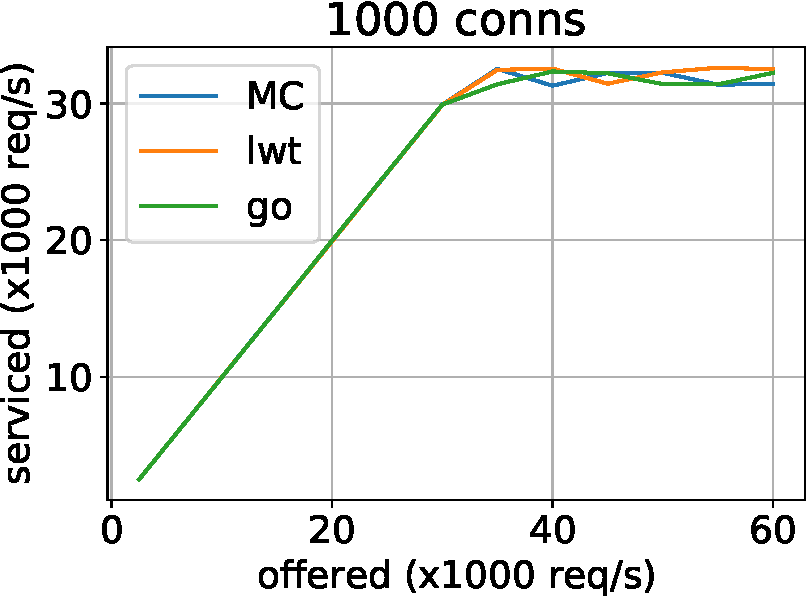
\includegraphics[width=0.9\linewidth]{http-benchmarks/throughput.pdf}
		\subcaption{Throughput}
		\label{grf:throughput}
	\end{minipage}
	\begin{minipage}{0.49\linewidth}
		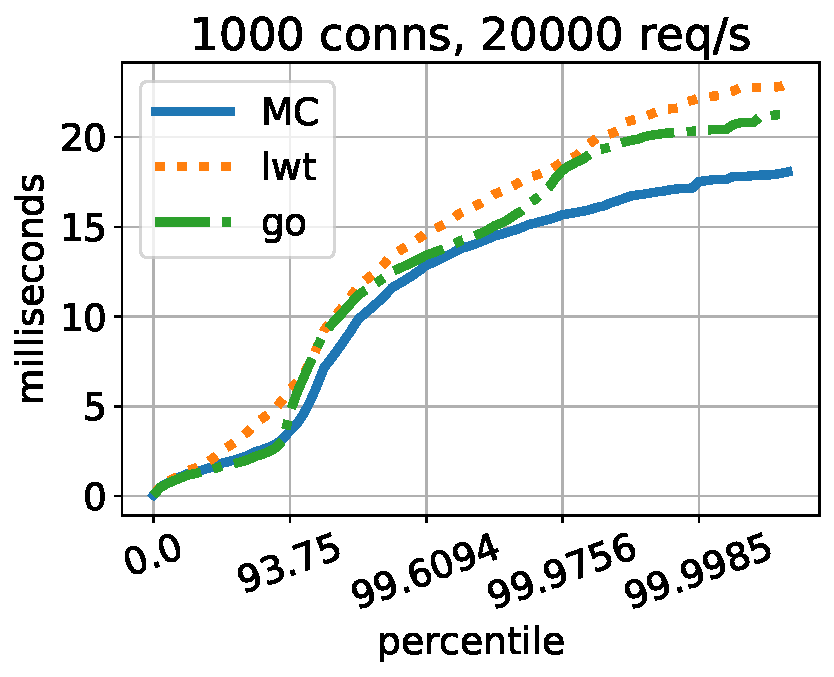
\includegraphics[width=0.9\linewidth]{http-benchmarks/latency.pdf}
		\subcaption{Tail latency}
		\label{grf:latency}
	\end{minipage}
	\vspace{-3mm}
	\caption{Web server performance.}
	\vspace{-5mm}
\end{figure}

The client workload was generated with \texttt{wrk2}~\cite{wrk2}. We maintain
1k open connections and perform requests for a static web page at different
rates, and record the service rate and latency. The throughput and tail latency
graphs are given in Figures~\ref{grf:throughput} and~\ref{grf:latency}. In all
the versions, the throughput plateaus at around 30k requests per second. We
measure the tail latencies at 2/3rd of this rate (20k requests per second) to
simulate optimal load. We observe that both of the OCaml versions remain
competitive with |go|, and |MC| performs best in terms of tail latency.

Using effect handlers in the web server also helps with debugging the system as
a whole. Multicore OCaml supports getting the backtrace of a continuation,
which is a minor extension to getting the current backtrace. We can use this
feature to dump the backtrace of all the user-level threads in the web server.
Such a feature is provided by Go~\cite{gopprof}, but not possible with OCaml
concurrency libraries such as Async and Lwt which lack the notion of a thread.

\vspace{-3.5mm}
\section{Related Work}
\label{sec:related}

There are several strategies for implementing effect handlers. Eff~\cite{Eff},
Helium~\cite{Biernacki20}, Frank~\cite{Frank}, Links server
backend~\cite{Hillerstrom20} use an interpreter similar to our operational
semantics to implement effect handlers. Effekt~\cite{Effekt}, Links JavaScript
backend~\cite{Hillerstrom20} and Koka~\cite{Leijen17} use type-directed
selective CPS translation. These language are equipped with an effect system,
which allows compiling pure code in direct-style and effectful code in CPS.
Leijen~\cite{Leijen14} implements effect handlers as a library in C using stack
copying. Since C allows pointers into the stack, care is taken to ensure that
when continuations are resumed, the constituent frames are restored to the same
memory addresses as at the time of capture. Kiselyov et al.~\cite{Kiselyov18}
use an implementation of multi-prompt delimited continuations as an OCaml
library~\cite{Kiselyov12} to embed Eff language in OCaml. Indeed, Forester et
al.~\cite{Forster19} showed that in an untyped setting, effect handlers,
monadic reflection and delimited control can macro-express each other.

Similar to~\cite{Leijen14, Kiselyov12}, Multicore OCaml uses the call stack for
implementing continuations, but our continuations are one-shot. Bruggeman et
al.~\cite{Bruggeman96} show how to implement one-shot continuations efficiently
using segmented stacks in Scheme. Farvardin et al.~\cite{Farvardin20} perform a
comprehensive evaluation of various implementation strategies for continuations
on modern hardware. Multicore OCaml stacks do not neatly fit the description of
one of these implementation strategies. They best described as using the resize
strategy from Farvardin et al. for each of the fibers, which are in turn linked
to represent the current stack and the captured continuations.

Kawahara et al.~\cite{Kawahara20} implement one-shot effect handlers using
coroutines as a macro-expressible translation, and present an embedding in Lua
and Ruby. Lua provides asymmetric coroutines~\cite{Lua} where each coroutine
uses its own stack similar to how each handled computation runs in its own
fiber in Multicore OCaml. Similar to Multicore OCaml, Lua does not allow
coroutines to include C frames. It is useful to note that Lua is an interpreted
language, unlike OCaml, and DWARF unwind tables are not a concern in Lua.

Multicore OCaml is not the first language to support stack inspection in the
presence of non-local control operators. Chez Scheme supports continuation
marks~\cite{Flatt20} which permit stack inspection as a language feature. This
enables implementation of dynamic binding, exceptions, profilers, debuggers,
etc, in the presence of first-class continuations. As the authors note,
continuation marks can be implemented using effect handlers, but direct support
for continuation marks leads to better performance. In this work, we focus on
retaining the support for stack inspection through DWARF unwind tables in the
presence of effect handlers.

The interaction of non-local control flow and resources has been studied
extensively. Scheme uses |dynamic-wind|~\cite{R5RS}, which is a generalisation of
Common Lisp |unwind-protect|~\cite{Steele90}, which ensures de-allocation (and
re-allocation) of resources every time the non-local control leaves and enters
back into a context. |dynamic-wind| is not quite what one wants for resource
clean up~\cite{Kiselyov,Sitaram03}. The main challenge is distinguishing
returning exits from non-returning ones. Resource clean up needs to occur only
during non-returning exit.

In Multicore OCaml, we build on the existing defensive coding practices against
exceptions to clean up resources on non-returning exits. Our continuations are
assumed to be resumed exactly once using |continue| or |discontinue|. As a
result, when a computation performs an effect, we are guaranteed that the
control will return. For the non-returning cases (value and exceptional
return), the code already handles resource cleanup. OCaml does not have a
\texttt{\footnotesize try/finally} construct commonly used for resource cleanup
in many programming languages. Alternative standard libraries such as
Base~\cite{BaseProtect} and Core~\cite{CoreProtect} provide mechanisms
analogous to |unwind-protect|, which are in turn implemented using exceptions.
Thus, the linear use of continuations enabled by the |discontinue| primitive
ensures backwards compatibility of legacy OCaml systems code under non-local
control flow introduced by effect handlers. Leijen~\cite{Leijen18} explicitly
extends effect handlers with |initially| and |finally| clauses in Koka for
resource safety.

Sivaramakrishnan et al.~\cite{TFP17} describe the interaction of effect
handlers and asynchronous exceptions. This is orthogonal to the contributions
of this paper. Our focus is the compiler and runtime system support for
implementing effect handlers.

\section{Conclusions}
\label{sec:conc}

We presented the motivation, design and implementation of effect handlers
specifically aimed at retrofitting them onto OCaml with tool compatibility,
negligible overheads for existing OCaml programs and good performance for those
that use effect handlers. Our evaluation shows that this is indeed the case.

\clearpage

\bibliographystyle{ACM-Reference-Format}
\bibliography{retro-concurrency}

\clearpage

\section*{Supplementary Material}
\setcounter{figure}{0}

\subsection*{Experimental support for multi-shot continuations}

Languages with effect handlers typically allow continuations to be resumed more
than once to enable use cases such as backtracking search and probabilistic
programming (Uber's Pyro langauge~\cite{Pyro}). Multicore OCaml has an
experimental feature for explicitly cloning continuations, which makes a copy
of each of its constituent fibers. Multi-shot continuations are difficult to
reason about in the presence of linear resources such as file descriptors.
Recall that OCaml programs are written with the expectation that function calls
return \emph{exactly-once} either normally or exceptionally. With multi-shot
continuations, they may return \emph{more than once}, leading to errors such as
double-freeing malloced memory. Since our goal is to retrofit effect handlers
onto OCaml, we relegate continuation cloning to the OCaml |Obj| module, which
contains unsafe features.

In addition, multi-shot continuations currently are not safe under compiler
optimisations. For example consider the following program:

\begin{minipage}{\linewidth}
\begin{lstlisting}
effect E : unit
let foo () = perform E
let bar f =
  let r = ref 0 in
	f ();
  r := !r + 1;
  !r
;;
match bar foo with
| v -> v
| effect E k ->
    let k' = Obj.clone_continuation k in
    let r1 = continue k () in
    let r2 = continue k' () in
    Printf.printf "%d %d\n" r1 r2;
		0
\end{lstlisting}
\end{minipage}

This program is expected to print |1 2|. However, OCaml optimizes |bar| by
converting the heap allocation of |r| to a stack allocation. As a result, each
continuation ends up with a copy of |r|, and the program prints |1 1|. Thus, in
the presence of multi-shot continuations, compiler optimisations need to be
made aware of the effects of a function. We leave proper support for multi-shot
continuations to future work.

\subsection*{No effect macro benchmarks}

\begin{figure*}
	\begin{minipage}{\linewidth}
	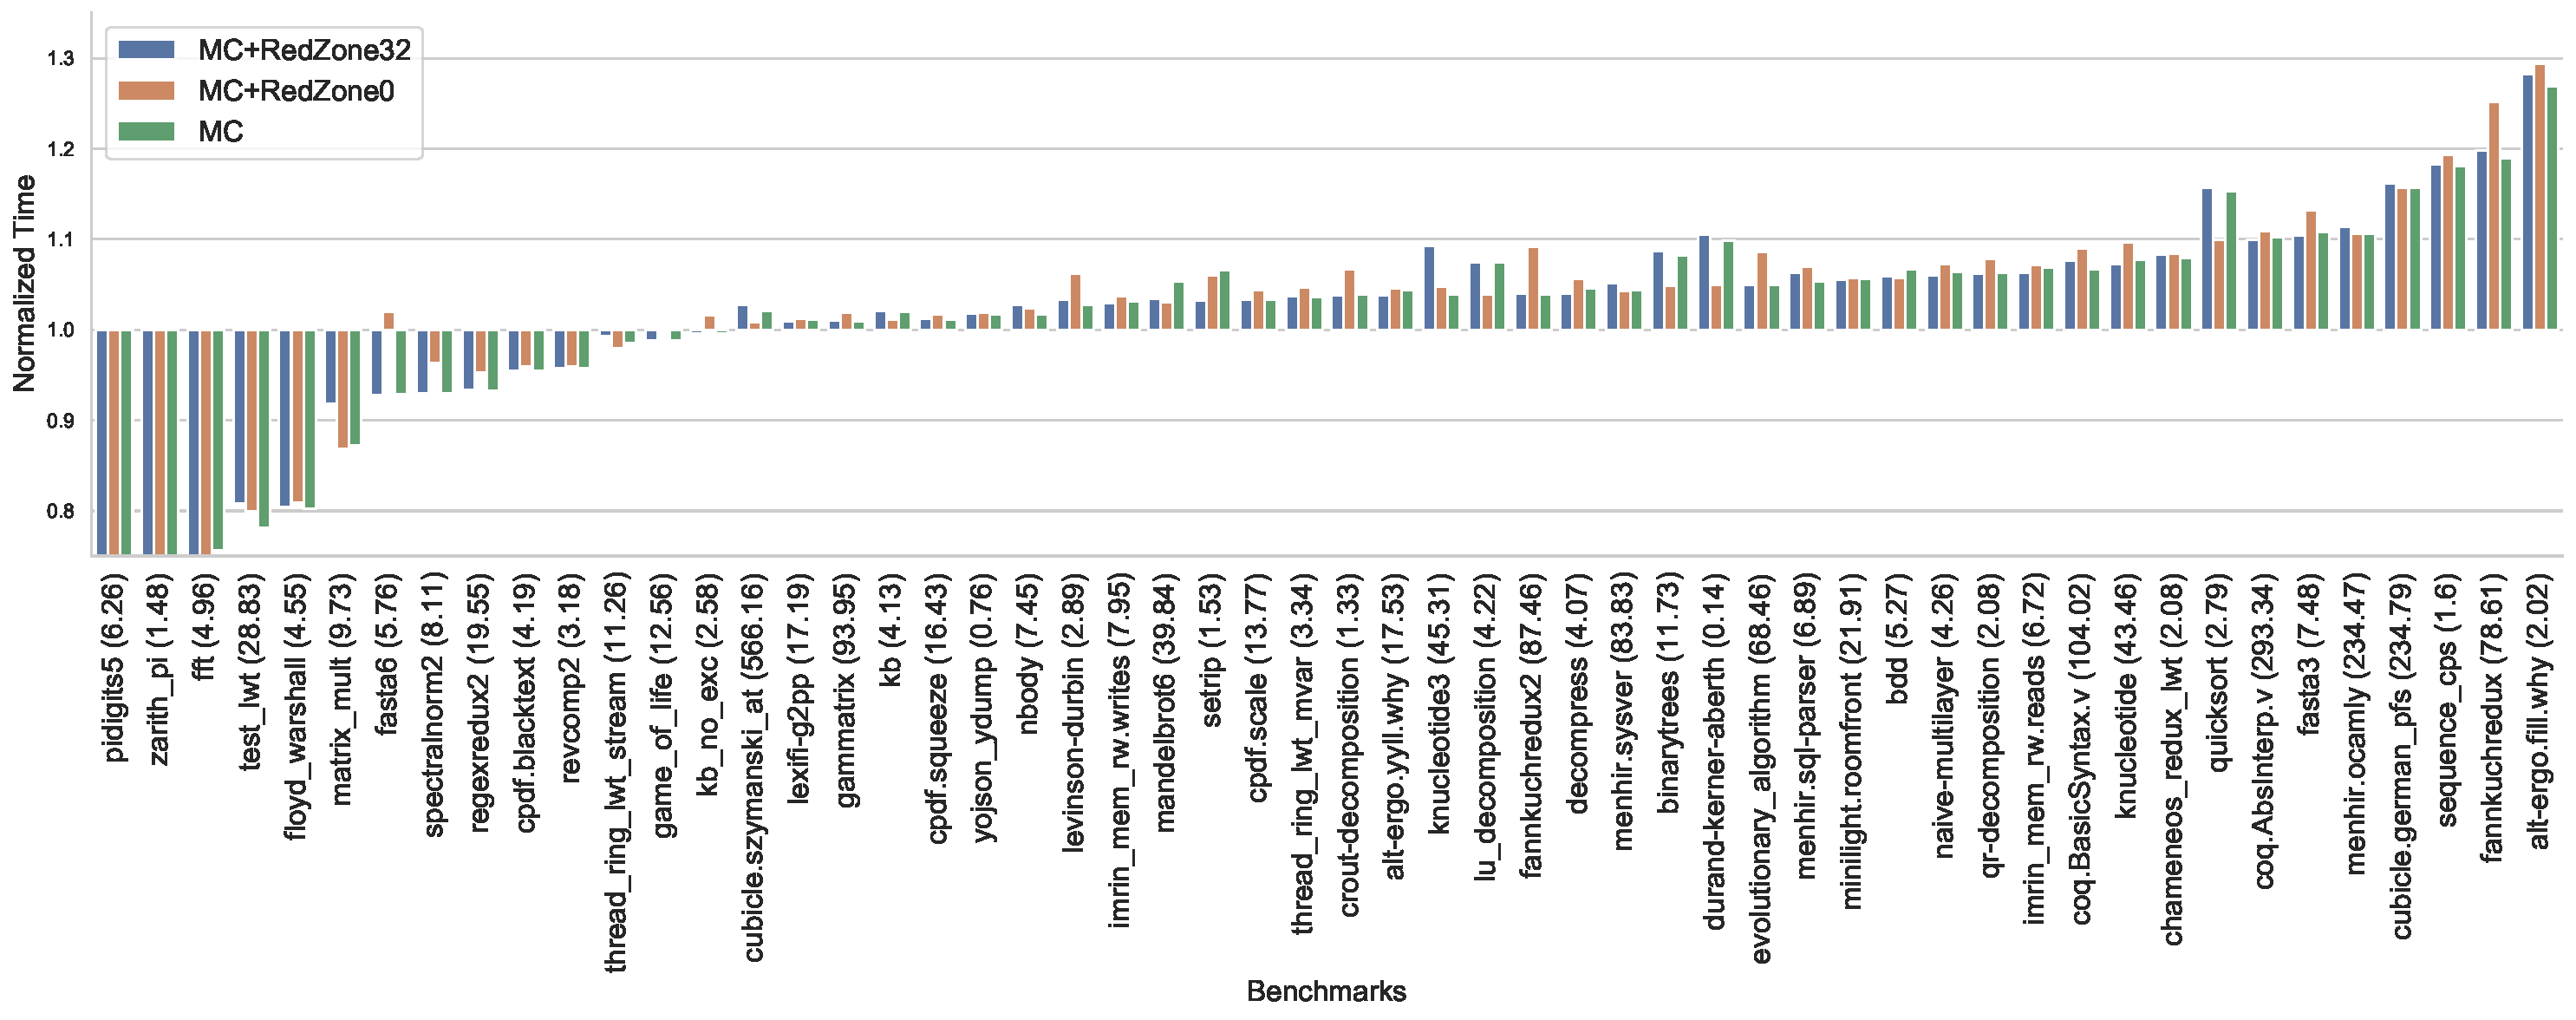
\includegraphics[width=\linewidth]{sandmark-notebook/sandmark_time}
	\subcaption{Normalized time of macro benchmarks. Baseline is Stock OCaml, whose running time in seconds in given in parenthesis.}
	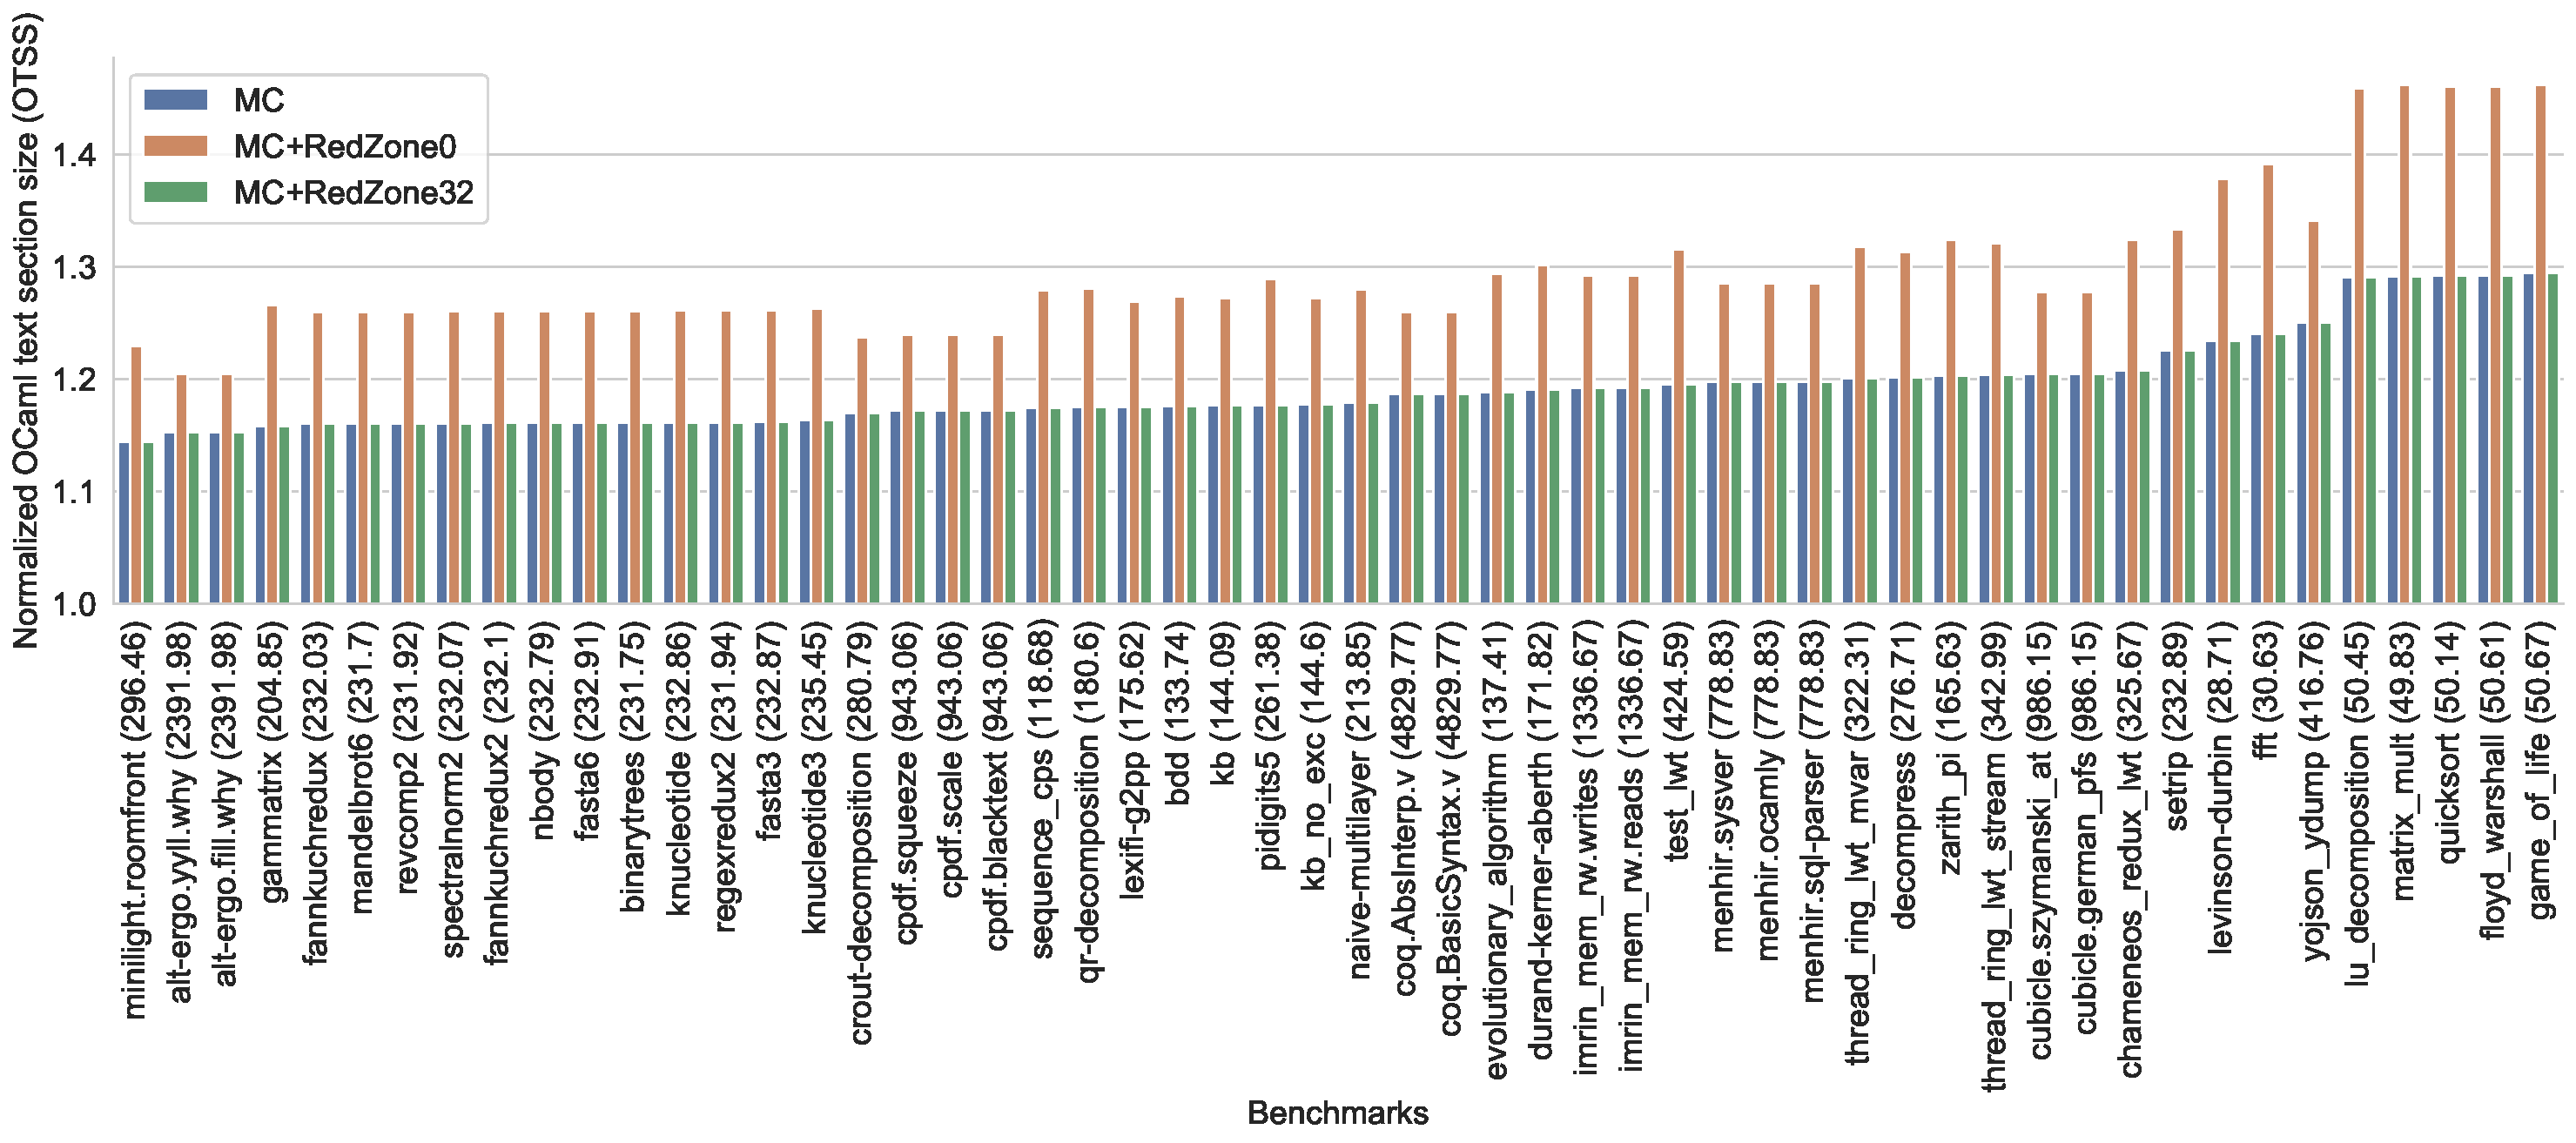
\includegraphics[width=\linewidth]{sandmark-notebook/sandmark_codesize}
	\subcaption{Normalized OCaml code size of macro benchmarks. Baseline is Stock OCaml, whose size in bytes given in parenthesis.}
	\end{minipage}
	\caption{Macro benchmark performance on code that does not use effects.}
	\label{res:macro}
\end{figure*}

Figure~\ref{res:macro} presents the performance of macro benchmarks that do not
use effects. The aim is to quantify the impact of the addition of effect
handlers to the language on code that does not use effect handlers. The |MC| is
Multicore OCaml with default red zone size (16 words). |MC+RedZone0| uses red
zone size of 0; every OCaml function has a stack overflow check. |MC+RedZone32|
uses a red zone size of 32 words.

\end{document}
